%\documentclass[twocolumns]{article}
\documentclass{article}%especifica o tipo de documento que tenciona escrever: carta, artigo, relatório... neste caso é um artigo

\usepackage[portuguese]{babel}%Babel -- irá activar automaticamente as regras apropriadas de hifenização para a língua todo o
                                   %-- o texto gerado é automaticamente traduzido para Português.
                                   %  Por exemplo, “chapter” irá passar a “capítulo”, “table of contents” a “conteúdo”.
                                   %portuges -- específica para o Português.
\usepackage[utf8]{inputenc} % define o encoding usado texto fonte (input)
\usepackage[T1]{fontenc}
\usepackage{ebproof}
% \usepackage{tikz} % Useless, but might be handy to draw fancier lines.
\usepackage{amssymb} % To provide the \varnothing symbol
\newcommand{\nothing}{\varnothing} % different from \emptyset
\usepackage{stmaryrd}

\begingroup
\catcode`[=\active \catcode`]=\active

% Define a meaning for active [ and ]
\gdef[{\llbracket} \gdef]{\rrbracket}

% Now take care of the \delcode of [ and ] for \left and \right
% First a temporary macro
\def\getdelim#1#2#3#4\relax{"#4}
% Use the temporary macro to get the right delcodes out of
% the meaning of \llbracket and \rrbracket
\global\delcode`[=\expandafter\getdelim\llbracket\relax
\global\delcode`]=\expandafter\getdelim\rrbracket\relax
\endgroup

% make [ and ] math active
\mathcode`\[="8000
\mathcode`\]="8000
\usepackage[table]{xcolor}
\usepackage{algpseudocode}
\usepackage{float}
\usepackage{hyperref}
\usepackage{graphicx} %permite incluir graficos, tabelas, figuras
\usepackage{listings}
\lstset{frame=tb,
  language=Haskell,
  aboveskip=3mm,
  belowskip=3mm,
  showstringspaces=false,
  columns=flexible,
  basicstyle={\small\ttfamily},
  breaklines=true,
  breakatwhitespace=true,
  tabsize=3,
 captionpos=b,
 inputencoding=utf8,
 extendedchars=true,
 literate={á}{{\'a}}1 {é}{{\'e }}1 {í}{{\'i}}1 {ó}{{\'o}}1 {ú}{{\'u}}1
  {Á}{{\'A}}1 {É}{{\'E}}1 {Í}{{\'I}}1 {Ó}{{\'O}}1 {Ú}{{\'U}}1
  {à}{{\`a}}1 {è}{{\`e}}1 {ì}{{\`i}}1 {ò}{{\`o}}1 {ù}{{\`u}}1
  {À}{{\`A}}1 {È}{{\'E}}1 {Ì}{{\`I}}1 {Ò}{{\`O}}1 {Ù}{{\`U}}1
  {ä}{{\"a}}1 {ë}{{\"e}}1 {ï}{{\"i}}1 {ö}{{\"o}}1 {ü}{{\"u}}1
  {Ä}{{\"A}}1 {Ë}{{\"E}}1 {Ï}{{\"I}}1 {Ö}{{\"O}}1 {Ü}{{\"U}}1
  {â}{{\^a}}1 {ê}{{\^e}}1 {î}{{\^i}}1 {ô}{{\^o}}1 {û}{{\^u}}1
  {Â}{{\^A}}1 {Ê}{{\^E}}1 {Î}{{\^I}}1 {Ô}{{\^O}}1 {Û}{{\^U}}1
  {ã}{{\~a}}1 {ẽ}{{\~e}}1 {ĩ}{{\~i}}1 {õ}{{\~o}}1 {ũ}{{\~u}}1
  {Ã}{{\~A}}1 {Ẽ}{{\~E}}1 {Ĩ}{{\~I}}1 {Õ}{{\~O}}1 {Ũ}{{\~U}}1
  {œ}{{\oe}}1 {Œ}{{\OE}}1 {æ}{{\ae}}1 {Æ}{{\AE}}1 {ß}{{\ss}}1
  {ű}{{\H{u}}}1 {Ű}{{\H{U}}}1 {ő}{{\H{o}}}1 {Ő}{{\H{O}}}1
  {ç}{{\c c}}1 {Ç}{{\c C}}1 {ø}{{\o}}1 {å}{{\r a}}1 {Å}{{\r A}}1
  {€}{{\euro}}1 {£}{{\pounds}}1 {«}{{\guillemotleft}}1
  {»}{{\guillemotright}}1 {ñ}{{\~n}}1 {Ñ}{{\~N}}1 {¿}{{?`}}1 {¡}{{!`}}1 
}

\parindent=0pt
\parskip=2pt


\title{Ultimate Fighting Championship Stats } %Titulo do documento
\author{Etienne Costa %define o nome do 1. autor
        \\Bruno Sousa
        
        \\ Universidade do Mihho %...e sua filiação
        
        \\Escola de Engenharia\\ Braga
 } %autores do documento
\date{ (\today)} %data



\begin{document} % corpo do documento

\maketitle %apresentar titulo, autor e data

\begin{abstract} % resumo do documento
\noindent O presente trabalho é referente a criação de um web site capaz de fornecer as estatísticas gerais do \textit{ufc} , que é a maior organização de artes marciais mistas e ainda ter a capacidade de prever resultados de diversas lutas, tirando partido de um base de dados semântica baseada em grafos, na qual será possível efectuar diversas queries em SPARQL .



\end{abstract}



\newpage
\section{Introduction} \label{sec:background}

O presente relatório é referente ao trabalho prático desenvolvido na Unidade Curricular \textit{Processamento e Representação de Conhecimento}, do 4° ano do Mestrado Integrado em Engenharia Informática da Universidade do Minho .

É pretendido com este trabalho prático desenvolver um sistema de consulta de dados estatísticos da maior organização de artes marciais mistas e ainda ter a capacidade de prever resultados de diversas lutas .

Para a realização deste projecto, serão utilizadas diversas ferramentas, por isso numa primeira fase será feita uma contextualização do problema e o conjunto de requisitos à alcançar . De seguida, é feita uma explicação mais detalhada de todo o processo de desenvolvimento,concretamente sobre a obtenção de dados, conversão de dados, funcionamento da arquitetura de todo o sistema,esmiuçando as respectivas componentes de ambos bem como os seus propósitos.

Por fim, será feita uma representação dos resultados obtidos, e uma conclusão perspectivando o trabalho futuro .


\section{Analysis and Specification}

\subsection{Project Description}

O projecto em questão consistiu no desenvolvimento de uma aplicação web para realizar consultas de dados estatísticos da maior organização de artes marciais mistas(\textit{UFC}), tendo ainda a possibilidade de prever o resultado de uma luta entre os lutadores presentes no sistema. Tendo sido selecionado um tema, foi necessário fazer a construção de uma ontologia sobre o tema selecionado de modo a armazenar a mesma no \textit{GraphDB}, que é uma base de dados de semântica baseada em grafos, na qual será possível efectuar diversas queries em \textit{SPARQL}.


\subsection{Requirement Specification}

O levantamento de requisitos é considerada a etapa mais importante, pois é nela que se priorizam as necessidades do futuros usuários do software, necessidades essas denominadas como \textit{requisitos}. Os principais requisitos levantados nesta etapa foram os seguintes :

\newpage
\textbf{Requisitos de descrição}:

\begin{itemize}
    \item Event :
    \begin{itemize}
        \item Name
        \item Date
    \end{itemize}
    \item Fight :
    \begin{itemize}
        \item (Red|Blue)CornerSigStr
        \item (Red|Blue)CornerSigStrPercentage
        \item (Red|Blue)CornerKD
        \item (Red|Blue)CornerTD
        \item (Red|Blue)CornerTDPercentage
        \item (Red|Blue)CornerResult
        \item (Red|Blue)CornerCTRL
        \item (Red|Blue)CornerReversal
        \item (Red|Blue)CornerTotalStrikes
        \item (Red|Blue)CornerSubAtt
        \item (Red|Blue)Corner
        \item Round
        \item Bout
        \item Method
        \item Time 
        \item TimeFormat
    \end{itemize}
    \item Fighter :
    \begin{itemize}
        \item Name
        \item Nickname
        \item DateOfBirth
        \item Weight
        \item Height
        \item Reach
        \item Stance
        \item Belt
        \item Wins
        \item Losses
        \item Draws
        \item Significant Strikes Absorbed per Minute
        \item Significant Strikes Landed per Minute
        \item Average Submissions Attempted per 15 minutes 
        \item Significant Strike Defence 
        \item Significant Striking Accuracy
        \item Takedown Accuracy 
        \item Average Takedowns Landed per 15 minutes 
        \item Takedown Defense 
    \end{itemize}
    \item Referee:
    \begin{itemize}
        \item Name
    \end{itemize}
    \item Location:
    \begin{itemize}
        \item Country
        \item City
        \item State

    \end{itemize}
\end{itemize}

\textbf{Requisitos de Exploração} :
\begin{itemize}
    \item Listar todos os eventos do sistema 
    \item Listar todas as lutas de um determinado evento
    \item Listar todas os lutadores do sistema
    \item Listar todas as lutas de um determinado lutador
    \item Listar as estatísticas gerais por carreira
    \item Listar as estatísticas gerais por luta 
    \item Listar as estatísticas gerais por evento
    \item Listar as estatísticas gerais por localização
    \item Listar as estatísticas gerais por arbitragem
    \item Listar os campeões actuais da organização
    \item Fazer a previsão de lutas entre dois lutadores
    \item Listar o resultado de todas as previsões efectuadas no sistema
    \item Listar as reviews feitas no sistema
    \item Listar as estatísticas gerais do repositório 
\end{itemize}


\newpage
\section{Web Scraping} \label{sec:background}

O conjunto de dados era um requisito primordial para a realização deste projecto, sendo que os mesmos podiam ser obtidos de inúmeras maneiras,e.g, \textbf{Linked Open Data Cloud},\textbf{Kaggle}, etc .\\ 

Contudo optou-se por ir no sentido inverso e testar as capacidades de produzir um ficheiro semiestruturado recorrendo ao web scraping .
O \textbf{web scraping} é uma solução para quem quer ter acesso a dados da web de uma forma automatizada, principalmente quando o site do qual se pretene obter dados não possuí uma API.\\

No contexto do nosso problema tivemos sempre presente a informação relevante a ser extraída,i.e, o conjunto de eventos decorridos no \textit{ufc} desde 1994 até ao ano corrente, bem como a informação de cada uma das lutas e dos seus intervenientes . 

Portanto seguiu-se o processo típico de web scrapping :

\begin{itemize}
    \item Identificar os websites
    \begin{itemize}
        \item  \url{http://ufcstats.com/statistics/events/completed}
        \item  \url{http://ufcstats.com/statistics/fighters}
        \item   \url{https://www.ufc.com/athletes/all}
    \end{itemize}
    
    \item Recolher URLs das páginas identificadas
    \item Fazer um pedido a estes URLs de modo a obter o HTML da página
    \item Utilizar localizadores para encontrar os dados em HTML
    \item Armazenar os dados num ficheiro JSON e CSV 
\end{itemize}

\subsection{Scripting}

A linguagem de programação escolhida para enfrentar este desafio foi o \textit{Python}, pois a mesma possuí diversas bibliotecas que nos auxiliam na execução de diversas tarefas,e.g., \textit{requests}, \textit{re}, \textit{json}, \textit{os}, \textit{time} e \textit{BeatifulSoutp} e além disso acaba por ser uma linguagem extremamente fácil para trabalhar.\\

Portanto optou-se por fazer 6 scripts, tendo cada um deles o seguinte objectivo :

\begin{itemize}
    \item events.py - responsável por obter toda a informação dos eventos e as suas respectivas lutas .
    \item fighters.py - responsável por obter a informação de todos os lutadores .
    \item face.py - responsável por obter as fotos de perfil existentes de todos os lutadores .
    \item full-body.py - responsável por obter as fotos de todos os lutadores .
    \item auxiliar.py - responsável por obter a quantidade de dados de modo a calcular a barra de progresso .
    \item ufc.py - script responsável por fundir toda informação e gerar um ficheiro semiestruturado .
\end{itemize}


\subsection{JavaScript Object Notaion}

A execução do \textit{ufc.py} permite-nos obter um json com o seguinte formato : 

\begin{lstlisting}[language=haskell, caption=Estrutura do json]
{
   "Referees":[
      {
         "Name":"Chris Tognoni"
      },
      {
         "Name":"Bill Clancy"
      },
      ". . ."
   ],
   "Fighters":[
      {
         "Name":"Khabib Nurmagomedov",
         "Nickname":"The Eagle",
         "Height":"5' 10",
         "Weight":"155 lbs",
         "Reach":70.0,
         "Stance":"Orthodox",
         "Wins":29,
         "Losses":0,
         "Draws":0,
         "Belt":"false",
         "DateOfBirth":"Sep 20 1988",
         "SLpM":4.1,
         "StrAcc":48.0,
         "SApM":1.75,
         "StrDef":65.0,
         "TDAvg":5.32,
         "TDAcc":48.0,
         "TDDef":84.0,
         "SubAvg":0.8
      },
      ". . ."
   ],
   "Events":[
      {
         "Name":"UFC_Fight_Night_Reyes_vs_Prochazka",
         "Location":{
            "City":"Las Vegas",
            "State":"Nevada",
            "Country":"USA"
         },
         "Date":"May 01 2021",
         "Fights":[
            {
               "Bout":"Light Heavyweight Bout",
               "RedCorner":"Dominick Reyes",
               "BlueCorner":"Jiri Prochazka",
               "RedCornerResult":"L",
               "BlueCornerResult":"W",
               "Method":"KO/TKO",
               "Round":"2",
               "Time":"4:29",
               "TimeFormat":"5 Rnd (5-5-5-5-5)",
               "Referee":"Herb Dean",
               "Stats":{
                  "RedCorner":{
                     "KD":"0",
                     "SigStr":"63 of 108",
                     "SigStrPercentage":"58%",
                     "TotalStrikes":"68 of 114",
                     "TD":"1 of 1",
                     "TDPercentage":"100%",
                     "SubAtt":"1",
                     "Reversal":"0",
                     "CTRL":"0:29"
                  },
                  "BlueCorner":{
                     "KD":"1",
                     "SigStr":"77 of 136",
                     "SigStrPercentage":"56%",
                     "TotalStrikes":"78 of 137",
                     "TD":"1 of 1",
                     "TDPercentage":"100%",
                     "SubAtt":"0",
                     "Reversal":"0",
                     "CTRL":"1:35"
                  }
               }
            },
            ". . ."
         ]
      },
      ". . ."
   ]
}              
\end{lstlisting}

\subsection{JSON Fields}

Alguns termos utilizados nos campos do json acabam por ser estranhos a quem não está familiarizado com o meio das lutas, portanto é feita uma breve tradução dos mesmos :

\begin{itemize}
    \item SLpM : Significant Strikes Landed Per Minute 
    \item StrAcc : Significant Striking Accuracy
    \item SApM : Significant Strikes Absorbed Per Minute
    \item StrDef :  Significant Strike Defence 
    \item TDAvg  :  Average Takedowns Landed Per 15 Minutes 
    \item TDAcc : Takedown Accuracy
    \item TDDef :  Takedown Defense 
    \item SubAvg :  Average Submissions Attempted per 15 minutes 
    \item KD : KnockDowns
    \item SigStr : Significant Strikes 
    \item SigStrPercentage : Significant Strikes Percentage 
    \item TD : Takedowns 
    \item TDPercentage : Takedowns Percentage 
    \item SubAtt : Submissions Attempted
    \item CTRL : Control Time
\end{itemize}

\subsection{Data Stats}

A organização do \textit{ufc} realiza eventos semanalmente, exigindo uma constante actualização da informação, portanto seria possível fazer uma execução semanal do nosso script de modo a obter os dados mais recentes, porém, visto que são feitos inúmeros pedidos para obter a informação dos eventos e lutadores o script leva um tempo considerável até obter toda informação então a versão apresentada neste momento foi obtida no dia 18 de Junho de 2021 tendo no total a seguinte informação :


\begin{table}[H]
\centering
\label{tab:my-table}
\begin{tabular}{|c|l|l|l|l|l}
\cline{1-5}
\textbf{Events} & \textbf{Fights}                    & \textbf{Fighters}                  & \textbf{Referees}                 & \textbf{Locations}                &  \\ \cline{1-5}
\textbf{565}    & \multicolumn{1}{c|}{\textbf{6149}} & \multicolumn{1}{c|}{\textbf{3664}} & \multicolumn{1}{c|}{\textbf{207}} & \multicolumn{1}{c|}{\textbf{166}} &  \\ \cline{1-5}
\end{tabular}
\caption{Overall Stats}

\end{table}

Informação essa calculada à custa de um pequeno script :

\begin{lstlisting}[language=python, caption= stats.py]
#!/usr/bin/python3

import json
with open('../web-scraping/JSON/ufc.json','r') as ufcfile:
    data = json.load(ufcfile)
    referees = data['Referees']
    fighters = data['Fighters']
    events = data['Events']
    fights = 0
    locations = []

    for e in events:
        if e['Location'] not in locations:
            locations.append(e['Location'])
        fights+=len(e['Fights'])

    print("Referees :: ",len(referees)) 
    print("Fighters :: ",len(fighters)) 
    print("Events :: ",len(events)) 
    print("Fights ::", fights) 
    print("Locations ::",len(locations)) 


\end{lstlisting}

\begin{figure}[H]
    \centering
    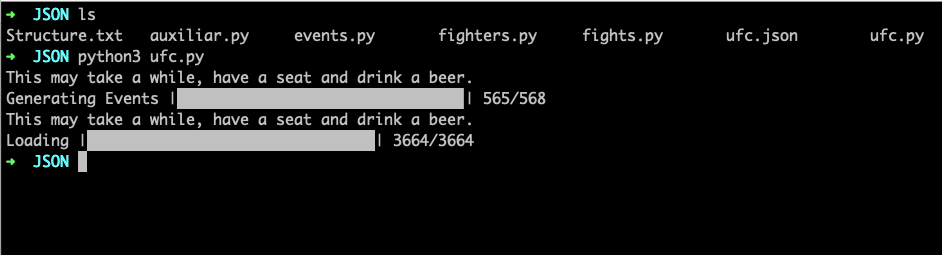
\includegraphics[width=1\textwidth]{imagens/Special Efects/Creating JSON.png}
    \caption{Creating JSON Script}
    \label{fig:mesh1}
\end{figure}





\newpage
\section{Ontology}

Uma ontologia é um modelo de dados que representa um conjunto de conceitos dentro
de um domínio e os relacionamentos entre estes, sendo que a mesma pode ser vista 
como uma especificação formal de conhecimento,i.e, capaz de ser compreendida por humanos e máquinas .\\
Ontologias geralmente descrevem :

\begin{itemize}
    \item Indivíduos : Objectos básicos 
    \item Classes : Conjuntos, coleções ou tipos de objectos 
    \item Atributos : Propriedade,características ou parâmetros que os objectos podem ter e compartilhar
    \item Relacionamentos : As formas como os objectos se podem relacionar com outros objectos 
\end{itemize}

\subsection{Specifying Ontologies}

Para especificar a nossa ontologia foram seguidas as seguintes metodologias:

\begin{enumerate}
    \item Especificação do domínio :
    \begin{itemize}
        \item Para que é que vamos usá-la?
        \item A que perguntas deve dar resposta?
        \item Quem vai usá-la e mantê-la ?
    \end{itemize}
    \item Enumeração dos termos mais importantes do domínio
    \item Definição das classes
    \item Definição dos atributos de cada classe
    \item Definição das relações entre indivíduos
    \item Definição dos indivíduos
\end{enumerate}

\subsubsection{Especificação do domínio}

A nossa ontologia foi definida com o propósito de proporcionar a informação pertinente do conjunto de atletas que pertencem ao \textit{ufc},i.e, providenciar um conjunto de dados estatísticos sobre todas as classes, podendo construir uma api capaz de consumir toda a informação da mesma e ainda conseguir fazer uma previsão de um possível resultado entre dois atletas com base nos seus atributos .\\
A manutenção da mesma será providenciada pelos seus criadores, tendo o cuidado de fazer um possível refactoring das queries em SPARQL de modo a não se perder o desempenho durante futuras consultas .

\subsubsection{Termos do domínio}

Tendo feito a especificação dos termos do nosso domínio, é possível identificar o conjunto de entidades, propriedades e relacionamentos entre os indivíduos .

\begin{figure}[!h]
    \centering
    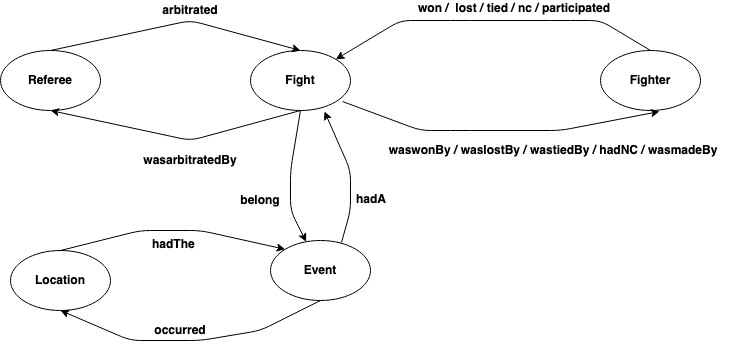
\includegraphics[width=1\textwidth]{imagens/Structure/ontology.png}
    \caption{Termos do domínio}
    \label{fig:mesh1}
\end{figure}



\begin{lstlisting}[language=Haskell, caption=Classes]
Classes :
                    - Event
                    - Fight
                    - Fighter
                    - Referee
                    - Location
\end{lstlisting}

\newpage
\begin{lstlisting}[language=Haskell, caption=Data Properties]
Data Properties :
                - Event :
                        - Date 
                        - Name
                - Fight :
                        - (Red|Blue)CornerSigStr
                        - (Red|Blue)CornerSigStrPercentage
                        - (Red|Blue)CornerKD
                        - (Red|Blue)CornerTD
                        - (Red|Blue)CornerTDPercentage
                        - (Red|Blue)CornerResult
                        - (Red|Blue)CornerCTRL
                        - (Red|Blue)CornerReversal
                        - (Red|Blue)CornerTotalStrikes
                        - (Red|Blue)CornerSubAtt
                        - (Red|Blue)Corner
                        - Round 
                        - Bout
                        - Method
                        - Time
                        - TimeFormat
                - Fighter :
                        - Name
                        - Nickname
                        - DateOfBirth
                        - Weight
                        - Height
                        - Reach
                        - Stance
                        - Belt
                        - Wins
                        - Losses
                        - Draws
                        - SApM
                        - SLpM
                        - SubAvg
                        - StrDef
                        - StrAcc
                        - TDAcc
                        - TDAvg
                        - TDDef
                - Referee :
                        - Name
                - Location :
                        - Country
                        - City
                        - State
\end{lstlisting}


\begin{lstlisting}[language=Haskell, caption=Object Properties]
Object Properties :

                    Pode ser interpretado como, um árbitro arbitrou uma luta, sendo o wasarbitratedBy a relação inversa .
                    
                    - arbitrated :      Referee --arbitrated--> Fight
                    - wasarbitratedBy : Fight --wasarbitratedBy--> Referee
                    
                    Pode ser interpretado como, um evento teve uma luta, sendo o belong a relação inversa .
                    
                    - hadA :   Event --hadA--> Fight
                    - belong : Fight --belong--> Event
                
                    Pode ser interpretado como, um fighter teve um 'no contest' numa luta, sendo o hadNC a relação inversa .
                
                    - nc :    Fighter --nc--> Fight
                    - hadNC : Fight --hadNC--> Fighter
                    
                    Pode ser interpretada como, um evento ocorreu numa localização, sendo o hadThe a relação inversa .
                    
                    - occurred : Event --occurred--> Location
                    - hadThe :   Location --hadThe--> Event
                    
                    Pode ser interpretada como, um lutador perdeu uma luta, sendo o waslostBy a relação inversa .
                    
                    - lost :      Fighter --lost--> Fight
                    - waslostBy : Fight --waslostBy--> Fighter
                    
                    Pode ser interpretada como, um lutador participou numa determinada luta, sendo o wasmadeBy a relação inversa .
                    
                    - participated : Fighter --participated--> Fight
                    - wasmadeBy :    Fight --wasmadeBy--> Fighter
                    
                    Pode ser interpretada como, um lutador empatou uma luta, sendo o wastiedBy a relação inversa .
                    
                    - tied :      Fighter --tied--> Fight
                    - wastiedBy : Fight --wastiedBy--> Fighter
                    
                    Pode ser interpretada como, um lutador ganhou uma luta, sendo o waswonBy a relação inversa .

                    - won :      Fighter --won--> Fight
                    - waswonBy : Fight --waswonBy--> Fighter
\end{lstlisting}




\subsection{Turtle}

O Resource Description Framework (RDF) é uma linguagem de propósito geral para representar informações na web.\\
Nesta secção é feita a conversão do json para um sintaxe textual de RDF chamada Turtle, que permite que um grafo RDF seja completamente escrito em um formato de texto compacto e natural, com abreviações para padrões de uso e tipos de dados comuns . 

\subsubsection{JSON To Turtle}

Para fazer a conversão fez-se a modelação do modelo base usando o Protégé , e de seguida implementou-se um script em python para fazer a geração do turtle.
Durante o processo de geração calculou-se a relação entre as classes num único sentido de modo a fazer a inferência das restantes relações no próprio Protégé .


\subsubsection{Extreme Cases}

Após a geração do ficheiro turtle, verificaram-se duas situações que comprometiam a utilização do mesmo. A primeira situação estava relacionada com o identificador dos lutadores, pois haviam 5 atletas que possuiam o mesmo nome e visto que nem sempre tínhamos as datas de nascimento, optou-se por fundir as lutas num único lutador e ficar com as data properties que pertencem ao segundo lutador encontrado .

\begin{lstlisting}[language=Haskell, caption=Repeated Names ]
Allow us to verify if the file have repeated names .

$ sort names.txt | uniq -d > repeated.txt 
$ cat repeated.txt 

Bruno Silva
Joey Gomez
Michael McDonald
Mike Davis
Tony Johnson
\end{lstlisting}

\newpage
A segunda situação está relacionada com o facto de no início da organização, haviam atletas que no mesmo evento podiam lutar duas vezes e estas lutas podiam assumir qualquer resultado, produzindo assim uma inconsistência no nosso turtle pois num determinado evento haviam lutas que apresentavam vários resultados.

\begin{figure}[H]
    \centering
    \vspace*{\fill}

% Your image goes here
\noindent
\makebox[\textwidth]{

    \fbox{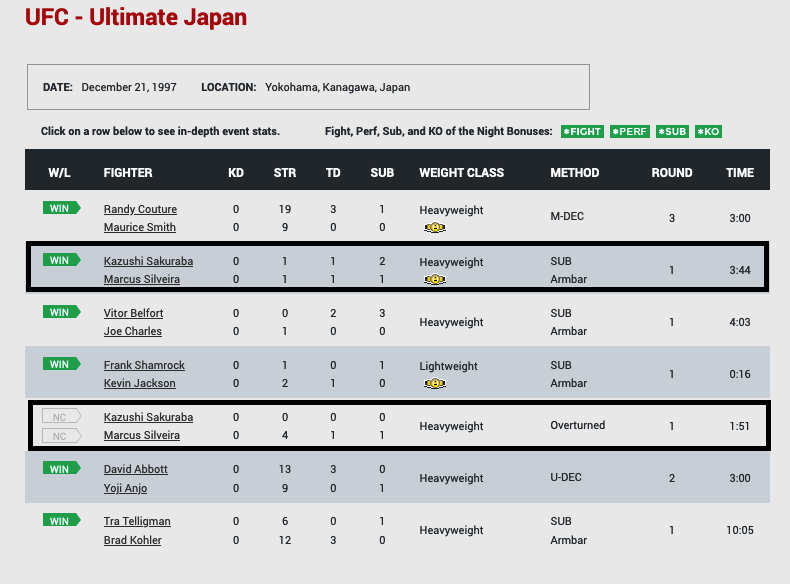
\includegraphics[scale=0.35]{imagens/Corner Cases/fightAtsameday.png}}
}%}

    \label{fig:my_label}
\end{figure}


\newpage
\section{API Server} 

O servidor que contém a API foi desenvolvido com o \textit{Node.js}, usando a framework de desenvolvimento \textit{Express.js}. Este servidor por sua vez está em constante comunicação o \textit{GraphDB}, visto que o mesmo possuí a nossa ontologia povoada . \\
Esta API servirá como ponto de ligação  dos end-users/aplicações à informação. \\
A mesma não se encontra protegida, porque o propósito é providenciar de forma aberta informações,estatísticas gerais e possíveis previsões de resultados aos principais amantes de artes marciais .

\begin{figure}[H]
    \centering
    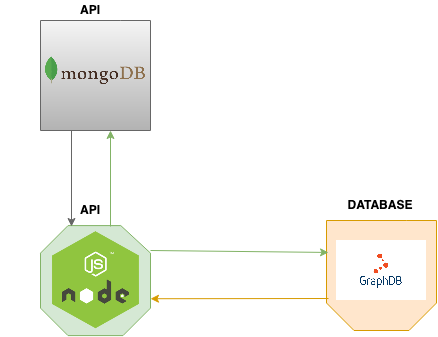
\includegraphics[width=1\textwidth]{imagens/Structure/API.png}
    \caption{Backend Structure}
    \label{fig:mesh1}
\end{figure}



\subsection{Rotas}

As rotas encaminham os pedidos dos clientes de forma a realizaram os pedidos a nossa base de dados, sendo que a rota para onde o utilizador é encaminhado varia consoante o URL e o método do pedido.

\begin{lstlisting}[language=python, caption= graphdb.js]
var prefixes = `
PREFIX : <http://www.di.uminho.pt/prc2021/ufc#>
PREFIX owl: <http://www.w3.org/2002/07/owl#>
PREFIX rdf: <http://www.w3.org/1999/02/22-rdf-syntax-ns#>
PREFIX xml: <http://www.w3.org/XML/1998/namespace>
PREFIX xsd: <http://www.w3.org/2001/XMLSchema#>
PREFIX rdfs: <http://www.w3.org/2000/01/rdf-schema#>`

exports.execQuery = async function (query){
    var getLink = "http://localhost:7200/repositories/UFC?query="
    var encoded = encodeURIComponent(prefixes + query)
    var result = await axios.get(getLink + encoded)
    return result.data
}
\end{lstlisting}




De seguida, apresentam-se as rotas definidas na nossa API : 


\textbf{Fighters: ufc/fighters}:

\begin{itemize}
    \item método GET
    \begin{itemize}
        \item \textbf{/} - Devolve a lista de lutadores no ufc com a sua respectiva informação pessoal .
        
        \item \textbf{/names} - Devolve a lista de nomes de todos os lutadores no ufc.
    \end{itemize}
\end{itemize}


\textbf{Fighter: ufc/fighter}:

\begin{itemize}
    \item método GET
    \begin{itemize}
        \item \textbf{/:id} - Devolve a informação pessoal de um determinado lutador.
        
        \item \textbf{/fights/:id} - Devolve todas as lutas de um determinado lutador.
    \end{itemize}
\end{itemize}

\textbf{Stats: ufc/stats}:

\begin{itemize}
    \item método GET
    \begin{itemize}
        \item \textbf{/career/ufc-fights} - Devolve o top 10 dos lutadores com mais lutas no ufc.
        
        \item \textbf{/career/mma-fights} - Devolve o top 10 dos lutas com mais lutas nas artes marciais mistas.
                

         \item \textbf{/career/wins} - Devolve o top 10 dos lutadores com mais vitórias no ufc.
        
         \item \textbf{/career/title-fight-wins} - Devolve o top 10 dos lutadores com mais vitórias em lutas por um título.
        
         \item \textbf{/career/KO-TKO} - Devolve o top 10 dos lutadores com mais vitórias por nocaute.
        
         \item \textbf{/career/submission-wins} -Devolve o top 10 dos lutadores com mais vitórias por submissão.
        
         \item \textbf{/career/finishes} - Devolve o top 10 dos lutadores com mais vitórias por finalização .
        
         \item \textbf{/career/decision} - Devolve o top 10 dos lutadores com mais vitórias por decisão .
        
         \item \textbf{/career/strike-accuracy} - Devolve o top 10 dos lutadores com melhor precisão a nível de golpes .
        
         \item \textbf{/career/strikes-landed-per-min} - Devolve o top 10 dos lutadores com mais golpes lançados por minutos .
        
         \item \textbf{/career/strike-defense} - Devolve o top 10 dos lutadores com maior precisão de golpes defendidos .
        
         \item \textbf{/career/takedown-accuracy} -  Devolve o top 10 dos lutadores com maior precisão de quedas .
        
         \item \textbf{/career/takedown-defense} - Devolve o top 10 dos lutadores com maior precisão de quedas defendidas .
        
         \item \textbf{/career/submission-average} - Devolve o top 10 dos lutadores com a melhor média de submissões .
        
         \item \textbf{/fight/fastest-finish} - Devolve o top 10 das lutas com menor duração .
         
        \item \textbf{/fight/fastest-KO-TKO} - Devolve o top 10 das lutas com menor duração terminas por um nocaute .
             
        \item \textbf{/fight/fastest-submission} - Devolve o top 10 das lutas com menor duração terminas por uma submissão .
        
        
        \item \textbf{/fight/latest-finish} - Devolve o top 10 das lutas com a finalização mais tardia .
          
          
        \item \textbf{/fight/latest-KO-TKO} - Devolve o top 10 das lutas com a finalização mais tardia por nocaute .
         
         
        \item \textbf{/fight/latest-submission} -  Devolve o top 10 das lutas com a finalização mais tardia por submissão .
         
         
        \item \textbf{/fight/knockdows-landed} -  Devolve o top 10 das lutas com nocautes .

         
         \item \textbf{/event/KO-TKO} - Devolve o top 10 dos eventos com maior número de lutas decididas por nocaute .
         
         \item \textbf{/event/submission-wins} - Devolve o top 10 dos eventos com maior número de lutas decididas por submissão .
         
         
         \item \textbf{/event/decision-wins} - Devolve o top 10 dos eventos com maior número de lutas decididas por pontos .
        
         \item \textbf{/location} - Devolve o top 10 das localizações com mais lutas  .
         
         \item \textbf{/referee} - Devolve o top 10 dos  árbitros com mais lutas arbitradas .
         
         
        \item\textbf{/titleholders} - Devolve a lista de campeões da organização .
      
    \end{itemize}
\end{itemize}


\textbf{Events: ufc/events}:

\begin{itemize}
    \item método GET
    \begin{itemize}
        \item \textbf{/} - Devolve a lista de eventos já realizados no ufc .
        
        \item \textbf{/details/:id} - Devolve os detalhes de um determinado evento .
        
        \item\textbf{/fights/:id} - Devolve as lutas de  um determinado evento .
      
    \end{itemize}
\end{itemize}



\textbf{Repository: /ufc/repositorie}:

\begin{itemize}
    \item método GET
    \begin{itemize}
        \item \textbf{/} - Devolve a informação do repositório .
    \end{itemize}
\end{itemize}



\newpage

\section{Predictions}

A comunidade que acompanha os grandes eventos de luta muita das vezes procura fazer o impossível, que é prever o resultado
de uma luta. O problema é que por natureza as lutas são extremamente imprevisíveis, o que torna as mesmas interessantes .

Portanto recorreu-se a um projecto na área de \textit{Machine Learning} desenvolvido por \textit{Charles Pierse} que tirando partido dos dados estáticos e dinâmicos dos lutadores constroí um sistema de previsão bi-direcional que funciona do seguinte modo : 

\begin{itemize}
    \item The first model uses the static stats as the independent variables for fighter 1 and fighter 2 and then predicts the dependent variables, the dynamic fight stats.( \textbf{multi target regression}).
    
    \item We then pass the static and dynamic fight stats to an overall winner model that predicts whether fighter 1 or fighter 2 is the winner. (\textbf{binary classification}).
    
\end{itemize}



\newpage







\section{Interface}

A interface foi desenvolvida através da framework \textit{Vue.js} e a framework de material \textit{Vuetify.js} baseada no \textit{Material Design da Google}. 

\begin{figure}[H]
    \centering
    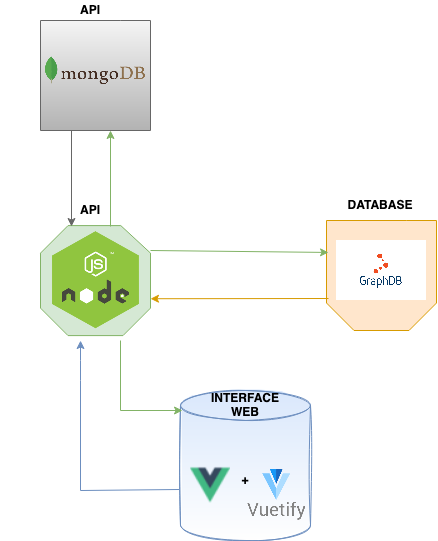
\includegraphics[width=1\textwidth]{imagens/Structure/structure.png}
    \caption{Backend and Frontend Structure}
    \label{fig:mesh1}
\end{figure}

Relativamente ao aspecto do website, procurou-se fazer uma implementação com um aspecto atrativo, recorrendo a inúmeras imagens descarregas durante o processo de \textit{scraping}, uma imagem na homepage com um dos maiores atletas da companhia e ícones anexados ao menu da navbar.

De seguida, serão apresentadas as diversas camadas da interface.



\subsection{Routes}

Nesta secção são apresentadas as rotas definidas :

\begin{lstlisting}[language=python, caption= Homepage route]
Rota associada a homepage, sendo feita a renderização da view Home.vue.

  { 
    path: '/', 
    redirect: { name: 'Home' }
  }
  ,
  {
    path: '/ufc',
    name: 'Home',
    component: Home,
  }
\end{lstlisting}


\begin{lstlisting}[language=python, caption= Fighters route]
Rota associada a página dos lutadores, sendo feita a renderização da view Fighters.vue.

{
   path: '/ufc/fighters',
    name: 'Fighters',
    // route level code-splitting
    // this generates a separate chunk (about.[hash].js) for this route
    // which is lazy-loaded when the route is visited.
    component: () => import(/* webpackChunkName: "about" */ '../views/Fighters.vue')
  }
\end{lstlisting}


\begin{lstlisting}[language=python, caption= Events route]
Rota associada a página dos eventos, sendo feita a renderização da view Events.vue.

  {
    path: '/ufc/events',
     name: 'Events',
     // route level code-splitting
     // this generates a separate chunk (about.[hash].js) for this route
     // which is lazy-loaded when the route is visited.
     component: () => import(/* webpackChunkName: "about" */ '../views/Events.vue')
   }
\end{lstlisting}


\begin{lstlisting}[language=python, caption= Homepage route]
Rota associada a página de um evento, sendo feita a renderização da view Event.vue.

   {
    path: '/ufc/event/:id',
     name: 'Event',
     // route level code-splitting
     // this generates a separate chunk (about.[hash].js) for this route
     // which is lazy-loaded when the route is visited.
     component: () => import(/* webpackChunkName: "about" */ '../views/Event.vue')
   }
\end{lstlisting}


\begin{lstlisting}[language=python, caption= Homepage route]
Rota associada a página de um lutador, sendo feita a renderização da view Fighter.vue.

{
    path: '/ufc/fighter/:id',
     name: 'Fighter',
     // route level code-splitting
     // this generates a separate chunk (about.[hash].js) for this route
     // which is lazy-loaded when the route is visited.
     component: () => import(/* webpackChunkName: "about" */ '../views/Fighter.vue')
   },
\end{lstlisting}

\begin{lstlisting}[language=python, caption= Homepage route]
Rota associada a página de previsões, sendo feita a renderização da view Predictions.vue.

  {
    path: '/ufc/predictions/',
     name: 'Predictions',
     // route level code-splitting
     // this generates a separate chunk (about.[hash].js) for this route
     // which is lazy-loaded when the route is visited.
     component: () => import(/* webpackChunkName: "about" */ '../views/Predictions.vue')
   }
\end{lstlisting}


\begin{lstlisting}[language=python, caption= Homepage route]
Rota associada a página com o histórico previsões, sendo feita a renderização da view PredictionsHistory.vue.

   {
    path: '/ufc/predictions/history',
     name: 'PredictionsHistory',
     // route level code-splitting
     // this generates a separate chunk (about.[hash].js) for this route
     // which is lazy-loaded when the route is visited.
     component: () => import(/* webpackChunkName: "about" */ '../views/PredictionsHistory.vue')
   }
\end{lstlisting}


\begin{lstlisting}[language=python, caption= Homepage route]
Rota associada a página de estatísticas gerais da companhia, sendo feita a renderização da view Stats.vue.

    {
    path: '/ufc/stats/',
     name: 'Stats',
     // route level code-splitting
     // this generates a separate chunk (about.[hash].js) for this route
     // which is lazy-loaded when the route is visited.
     component: () => import(/* webpackChunkName: "about" */ '../views/Stats.vue')
   }
\end{lstlisting}


\begin{lstlisting}[language=python, caption= Homepage route]
Rota associada a página de registo de avaliações gerais da aplicação, sendo feita a renderização da view RateUs.vue.

   {
    path: '/ufc/rate-us',
     name: 'Rate',
     // route level code-splitting
     // this generates a separate chunk (about.[hash].js) for this route
     // which is lazy-loaded when the route is visited.
     component: () => import(/* webpackChunkName: "about" */ '../views/RateUs.vue')
   }
\end{lstlisting}


\begin{lstlisting}[language=python, caption= Homepage route]
Rota associada a página de avaliações efectuadas da aplicação, sendo feita a renderização da view Reviews.vue.

   {
    path: '/ufc/reviews',
     name: 'Review',
     // route level code-splitting
     // this generates a separate chunk (about.[hash].js) for this route
     // which is lazy-loaded when the route is visited.
     component: () => import(/* webpackChunkName: "about" */ '../views/Reviews.vue')
   }
\end{lstlisting}


\begin{lstlisting}[language=python, caption= Homepage route]
Rota associada a página de estatísticas gerais do repositório, sendo feita a renderização da view Ontology.vue.

   {
    path: '/ufc/ontology/details',
     name: 'Ontology',
     // route level code-splitting
     // this generates a separate chunk (about.[hash].js) for this route
     // which is lazy-loaded when the route is visited.
     component: () => import(/* webpackChunkName: "about" */ '../views/Ontology.vue')
   }
\end{lstlisting}



\begin{lstlisting}[language=python, caption= Homepage route]
Permite identificar um url inválido na aplicação, renderizando a página com o erro associado (404) .
   {
    path: '*',
     name: 'PageNotFound',
     // route level code-splitting
     // this generates a separate chunk (about.[hash].js) for this route
     // which is lazy-loaded when the route is visited.
     component: () => import(/* webpackChunkName: "about" */ '../views/PageNotFound.vue')
   }

\end{lstlisting}

\subsection{Views}

Nesta secção são apresentadas as views definidas :

\begin{lstlisting}[language=python, caption= Home.vue]
Home.vue : 

    Está é a vista inicial com qual o utilizador tem a primeira interação, a mesma contém uma navbar e um footer, sendo que estes últimos são fixos,i.e, aparecem em todas as views implementadas. Também foi adicionado um vídeo com alguns highlights das lutas.

\end{lstlisting}


\begin{lstlisting}[language=python, caption= Fighters.vue]
Fighters.vue : 
    
    Nesta vista é possível ver uma tabela com a informação de todos os lutadores, sendo possível fazer pesquisas por qualquer um dos campos presentes no cabeçalho. Alguns dados como height,weight e stance podem ser convertidos para unidades mais convencionais,e.g, lbs par kg .

\end{lstlisting}

\begin{lstlisting}[language=python, caption= Fighter.vue]
Fighter.vue : 
    
    Nesta vista é possível ver o cartel actual do lutador,bem como os dados estáticos e dinâmicos do mesmo.
    Durante o processo de scraping, foram descarregadas algumas imagens e caso o lutador tenha uma imagem é feita o display da mesma. 
    Por baixo destas informações conseguimos consultar todas as lutas que o mesmo participou dentro da organização .
    
\end{lstlisting}


\begin{lstlisting}[language=python, caption= Events.vue]
Events.vue : 
    
    Nesta vista é possível ver uma tabela com a informação de todos os eventos, sendo possível fazer pesquisas por qualquer um dos campos presentes no cabeçalho. 
\end{lstlisting}


\begin{lstlisting}[language=python, caption= Event.vue]
Event.vue : 
    
    Nesta vista é possível ver a informação detalhada de um evento em específico,i.e, a data e a localização onde decorreu o evento, bem com a informação de todas as lutas que aconteceram neste evento. 
    
\end{lstlisting}


 
 \begin{lstlisting}[language=python, caption= Stats.vue]
Stats.vue : 

    Esta vista acaba por ser aquela que processa a maior quantidade de informação face ao número de pedidos que são feitos na nossa API, nela é possível consultar as estatísticas gerais da companhia sendo que as mesmas estão divididas em 5 categorias distintas.
    

\end{lstlisting}


 \begin{lstlisting}[language=python, caption= Predictions.vue]
Predictions.vue : 

    Nesta view é possível ver a listagem dos nomes dos lutadores, sendo obrigatório selecionar 2 lutadores de modo a conseguir fazer uma previsão do resultado de uma luta .
    Durante o processo de scraping foram descarregadas imagens dos lutadores, caso os lutadores selecionados possuam uma imagem é feito o display delas .
    
\end{lstlisting}

\begin{lstlisting}[language=python, caption= Ontology.vue]
Ontology.vue : 

    Nesta view é possível consultar alguma informação do repositório criado no graphDB .
    
\end{lstlisting} 


\begin{lstlisting}[language=python, caption= PredictionsHistory.vue]
PredictionsHistory.vue : 

    Nesta view é possível consultar o histórico de previsões efectuadas no sistema, visto que as mesmas podem ir mudando com as actualizações efectuadas no sistema .
    
\end{lstlisting} 

\begin{lstlisting}[language=python, caption= RateUS.vue]
RateUS.vue : 

    Nesta view é possível dar um feedback a aplicação, caso sejam fornercidos dados validados pelo formulário disponível .
    
\end{lstlisting}

\begin{lstlisting}[language=python, caption= Reviews.vue]
Reviews.vue : 

    Nesta view é possível consultar todo o feedback dado ao sistema, sendo que no mesmo aparecem a informação aparece ordenada pela data.
\end{lstlisting}


\begin{lstlisting}[language=python, caption= PageNotFound.vue]
PageNotFound.vue : 

    Nesta view é disponibilizada a representação de uma rota inexistente no sistema,i.e, 404 Page Not Found .
\end{lstlisting}

\newpage
\subsection{Results}

\begin{figure}[H]
    \centering
    
\includegraphics[width=1\textwidth]{imagens/HomePage/homepage1.png}
    \caption{Home Page Header}
    \label{fig:mesh1}
\end{figure}

\begin{figure}[H]
    \centering
    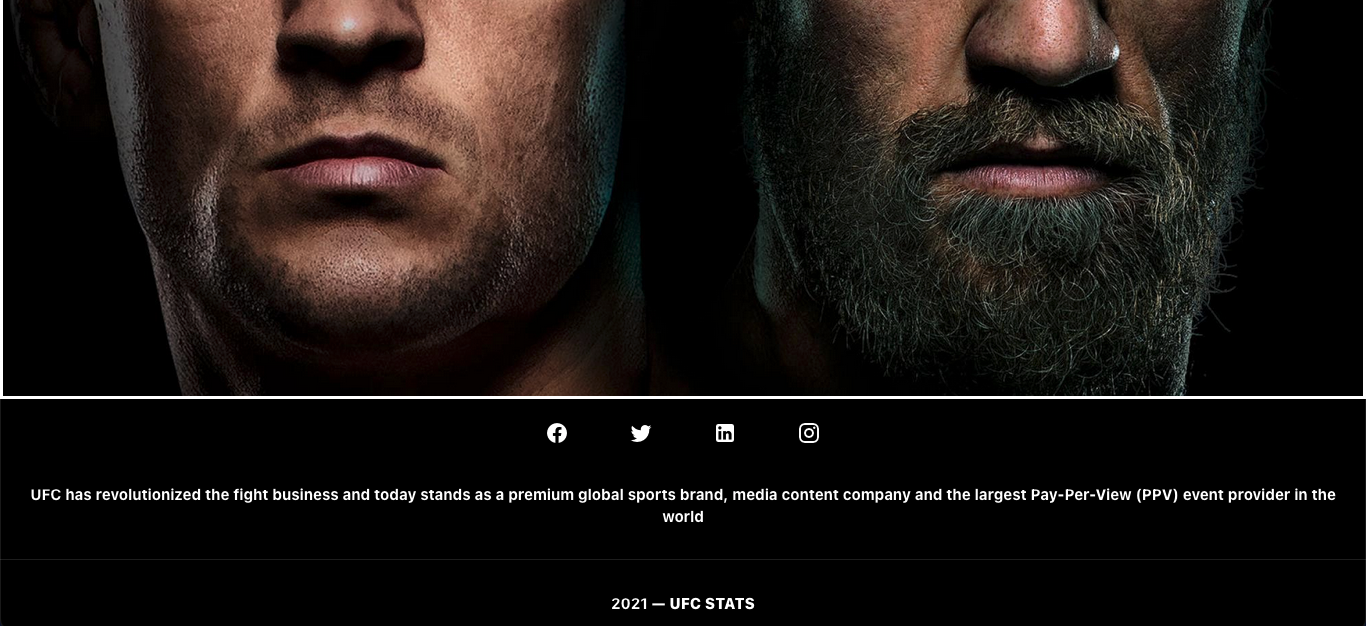
\includegraphics[width=1\textwidth]{imagens/HomePage/homepage2.png}
    \caption{Home Page Footer}
    \label{fig:mesh1}
\end{figure}

\begin{figure}[H]
    \centering
    
\includegraphics[width=1\textwidth]{imagens/HomePage/NavBar.png}
    \caption{Navigation Bar}
    \label{fig:mesh1}
\end{figure}


\begin{figure}[H]
    \centering
    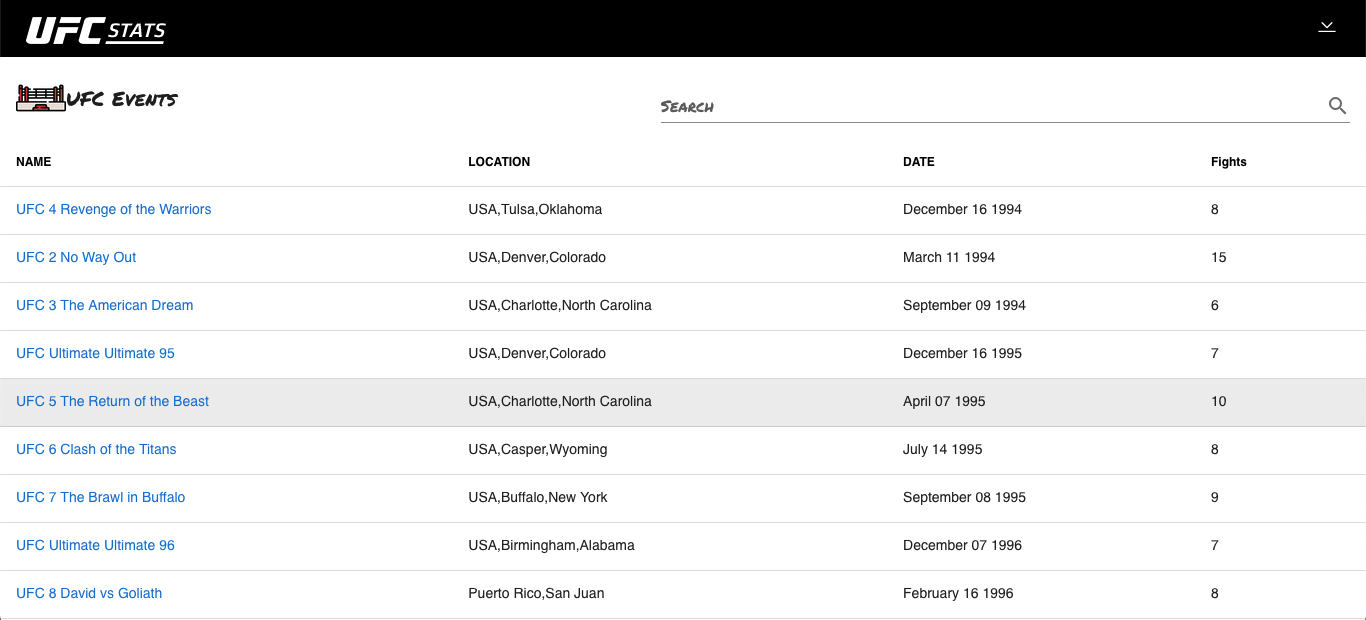
\includegraphics[width=1\textwidth]{imagens/Events/Events.png}
    \caption{Events}
    \label{fig:mesh1}
\end{figure}


\begin{figure}[H]
    \centering
    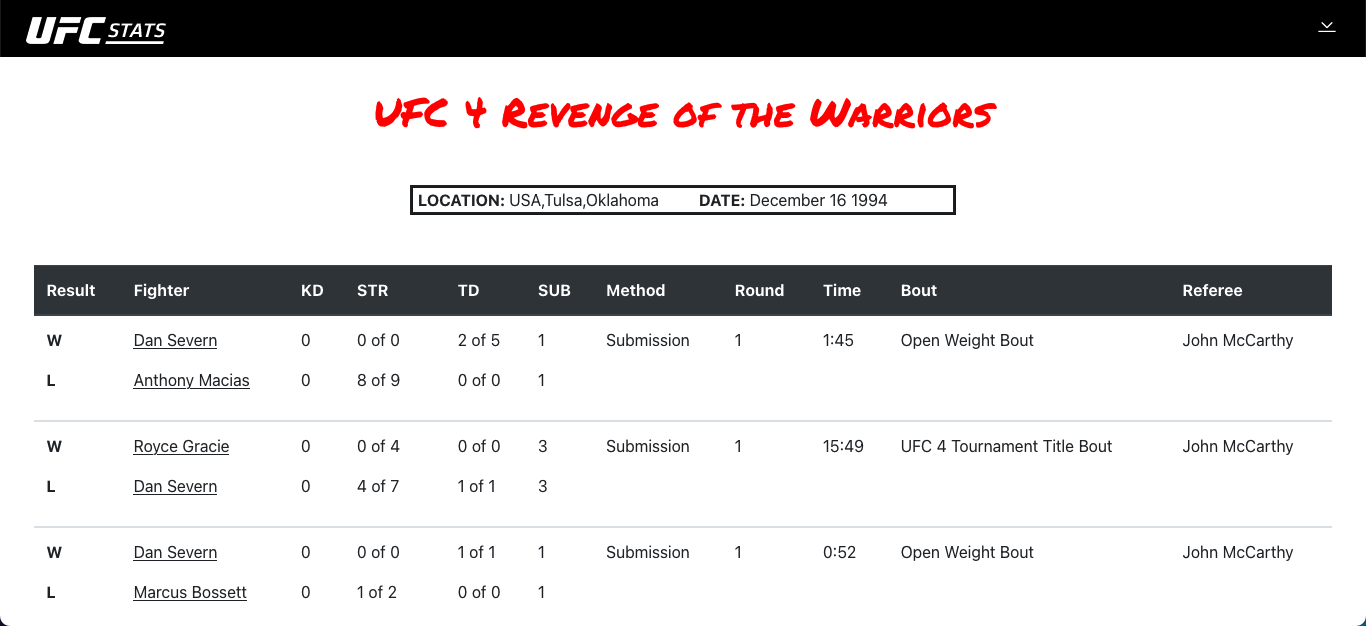
\includegraphics[width=1\textwidth]{imagens/Events/Event.png}
    \caption{Event}
    \label{fig:mesh1}
\end{figure}

\begin{figure}[H]
    \centering
    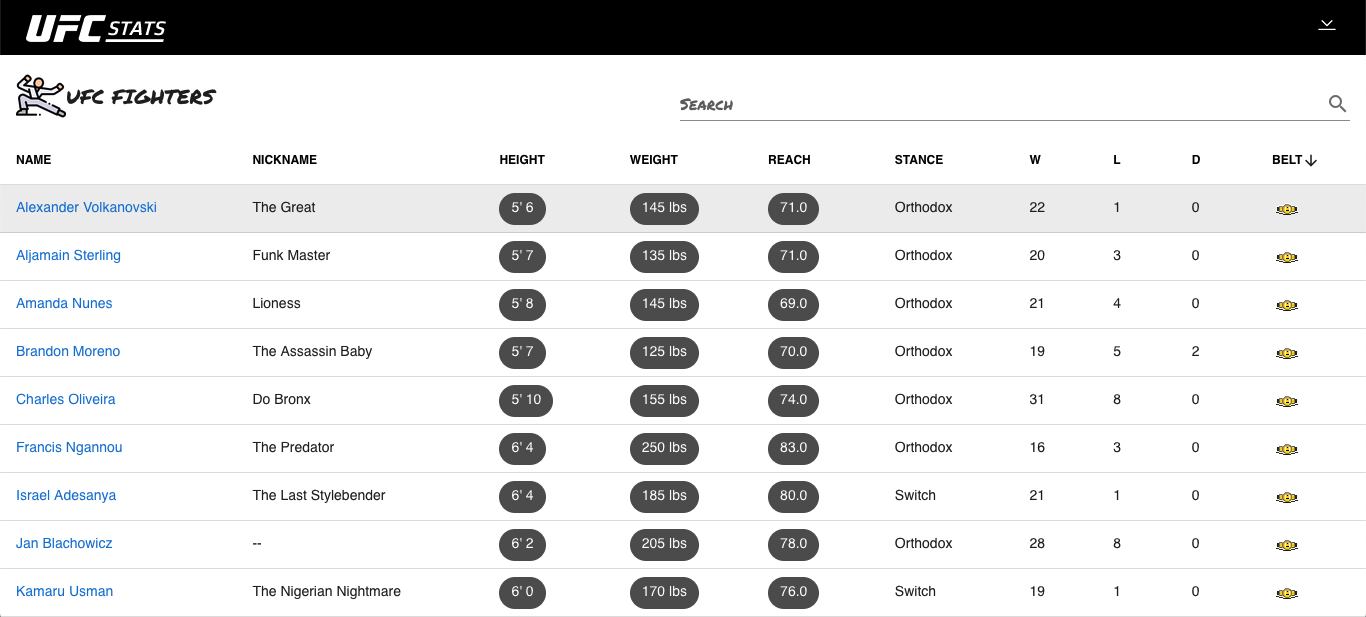
\includegraphics[width=1\textwidth]{imagens/Fighters/Fighters.png}
    \caption{Fighters}
    \label{fig:mesh1}
\end{figure}


\begin{figure}[H]
    \centering
    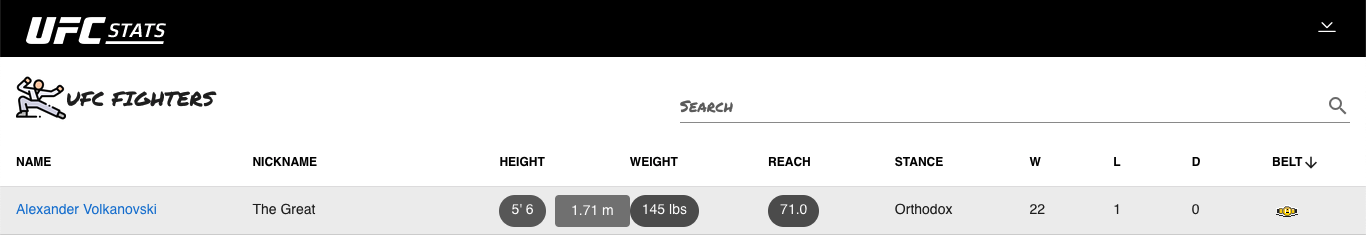
\includegraphics[width=1\textwidth]{imagens/Special Efects/Tooltip Weight.png}
    \caption{Tooltip Weight}
    \label{fig:mesh1}
\end{figure}


\begin{figure}[H]
    \centering
    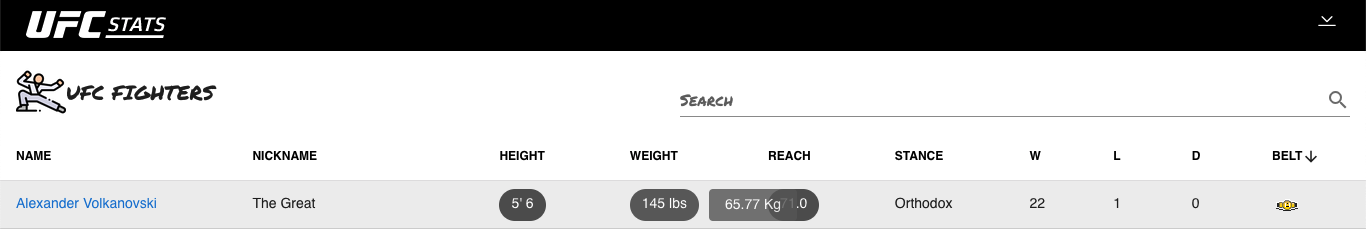
\includegraphics[width=1\textwidth]{imagens/Special Efects/Tooltip Height.png}
    \caption{Tooltip Height}
    \label{fig:mesh1}
\end{figure}

\begin{figure}[H]
    \centering
    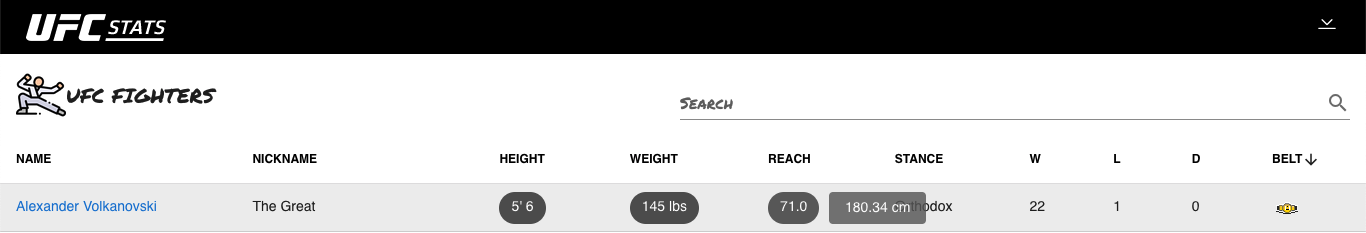
\includegraphics[width=1\textwidth]{imagens/Special Efects/Tooltip Reach.png}
    \caption{Tooltip Reach}
    \label{fig:mesh1}
\end{figure}

\begin{figure}[H]
    \centering
    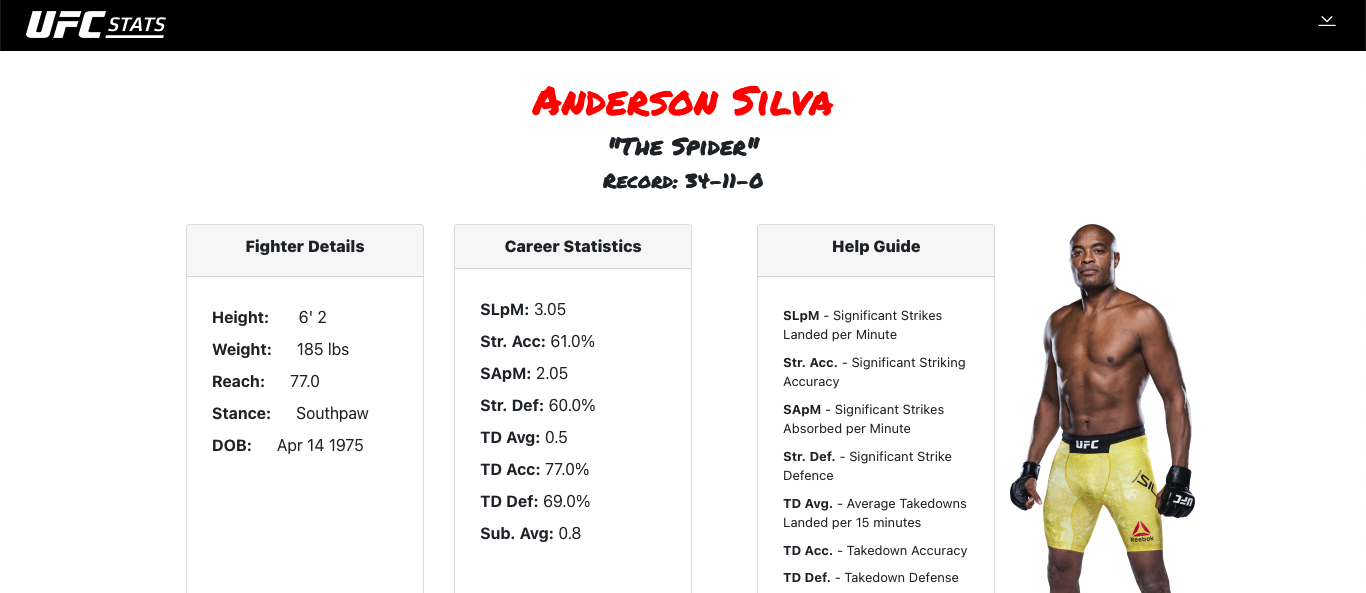
\includegraphics[width=1\textwidth]{imagens/Fighters/Anderson Silva.png}
    \caption{Anderson Silva - Fighter Details}
    \label{fig:mesh1}
\end{figure}


\begin{figure}[H]
    \centering
    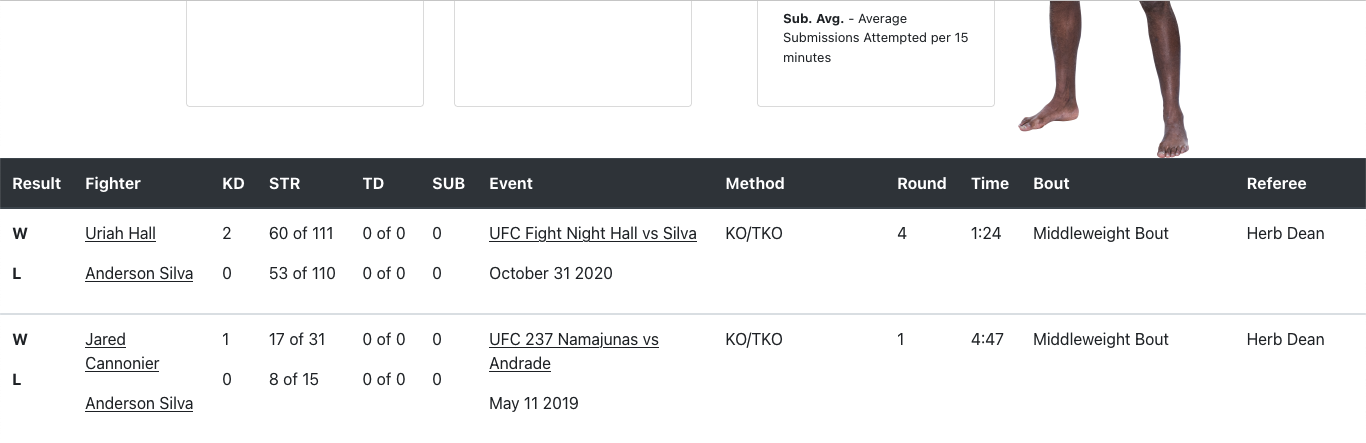
\includegraphics[width=1\textwidth]{imagens/Fighters/Anderson Silva2.png}
    \caption{Anderson Silva - Fighter Details 2}
    \label{fig:mesh1}
\end{figure}




\begin{figure}[H]
    \centering
    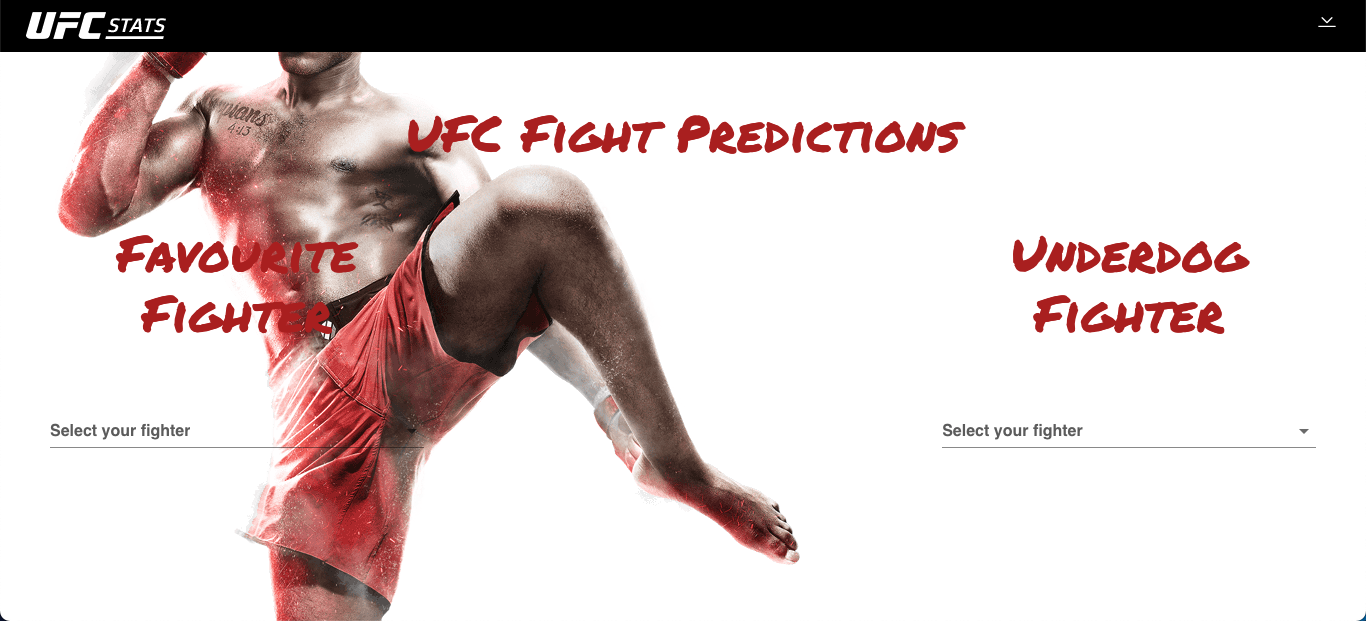
\includegraphics[width=1\textwidth]{imagens/Predictions/Predictions.png}
    \caption{Predictions}
    \label{fig:mesh1}
\end{figure}


\begin{figure}[H]
    \centering
    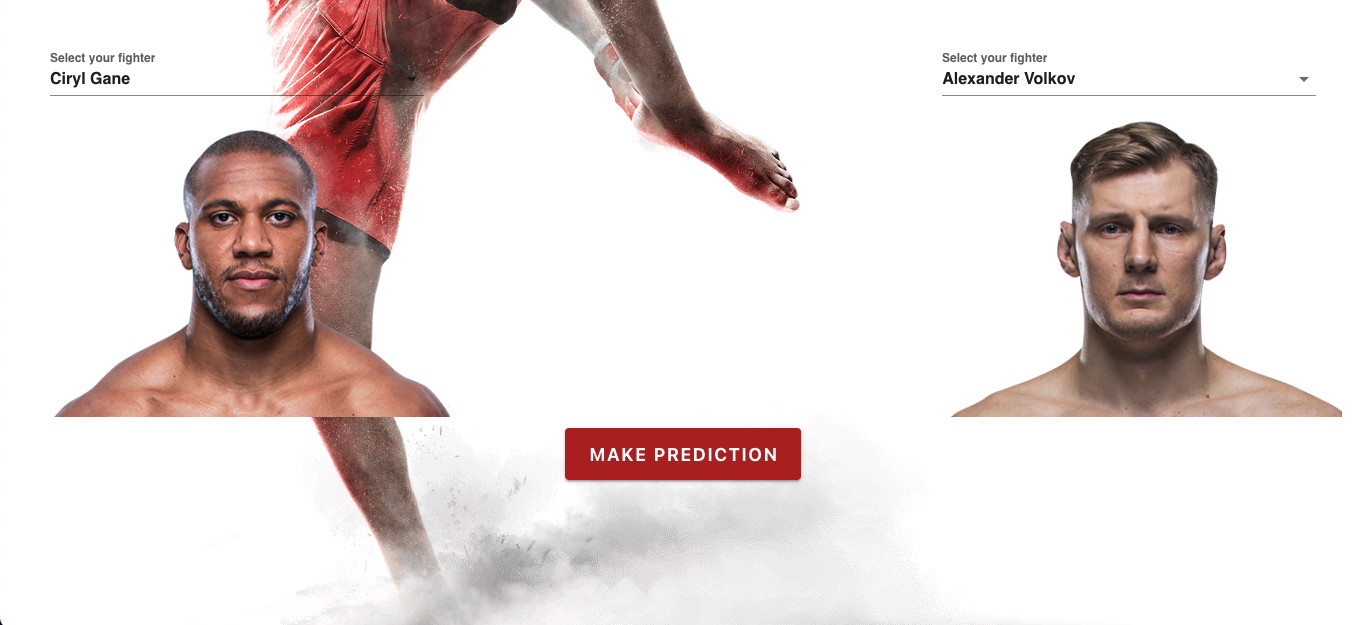
\includegraphics[width=1\textwidth]{imagens/Predictions/Predictions 2.png}
    \caption{Predictions 2 }
    \label{fig:mesh1}
\end{figure}



\begin{figure}[H]
    \centering
    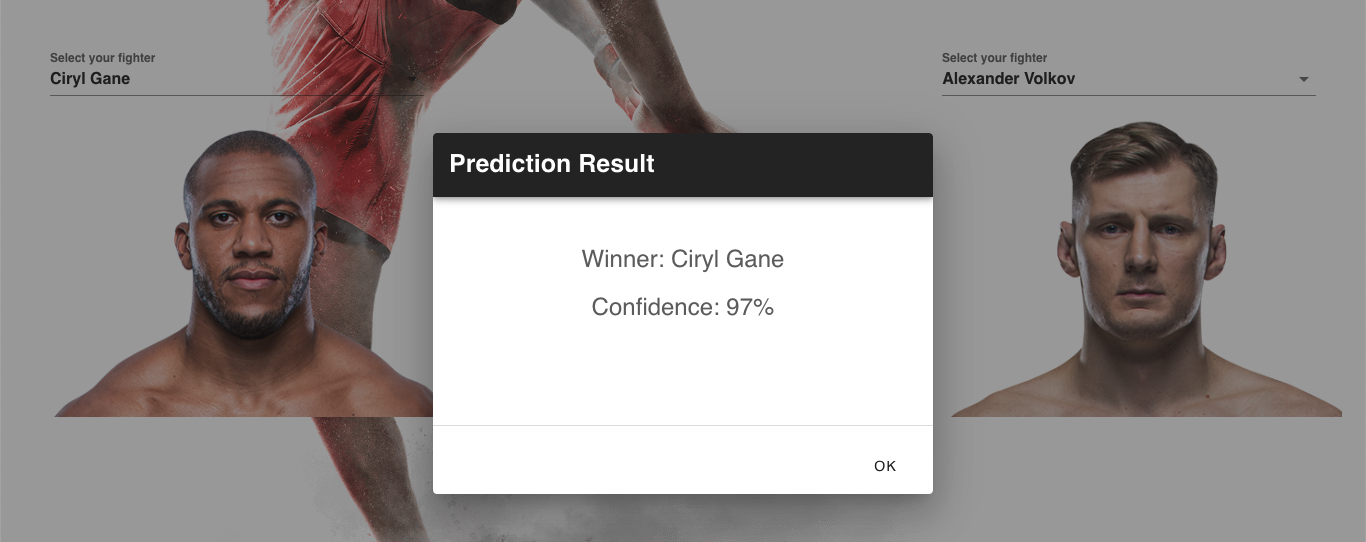
\includegraphics[width=1\textwidth]{imagens/Predictions/Prediction Result.png}
    \caption{Prediction Result}
    \label{fig:mesh1}
\end{figure}


\begin{figure}[H]
    \centering
    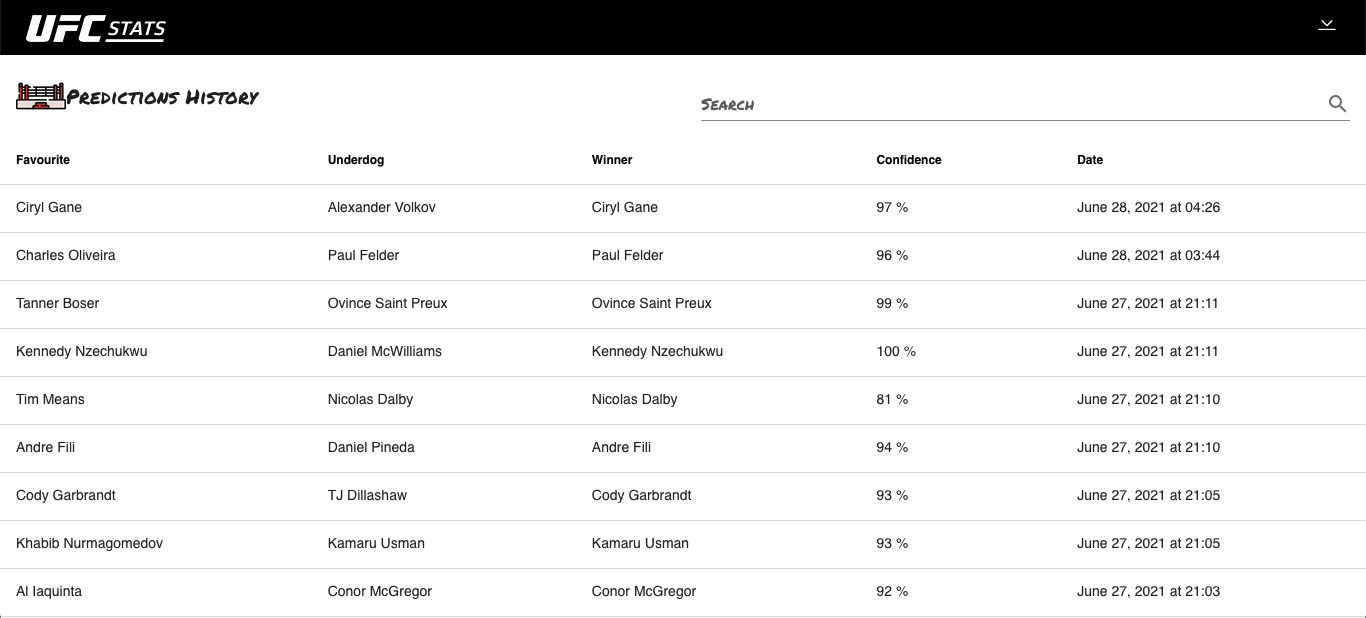
\includegraphics[width=1\textwidth]{imagens/Predictions/Prediction History.png}
    \caption{Prediction History}
    \label{fig:mesh1}
\end{figure}

\begin{figure}[H]
    \centering
    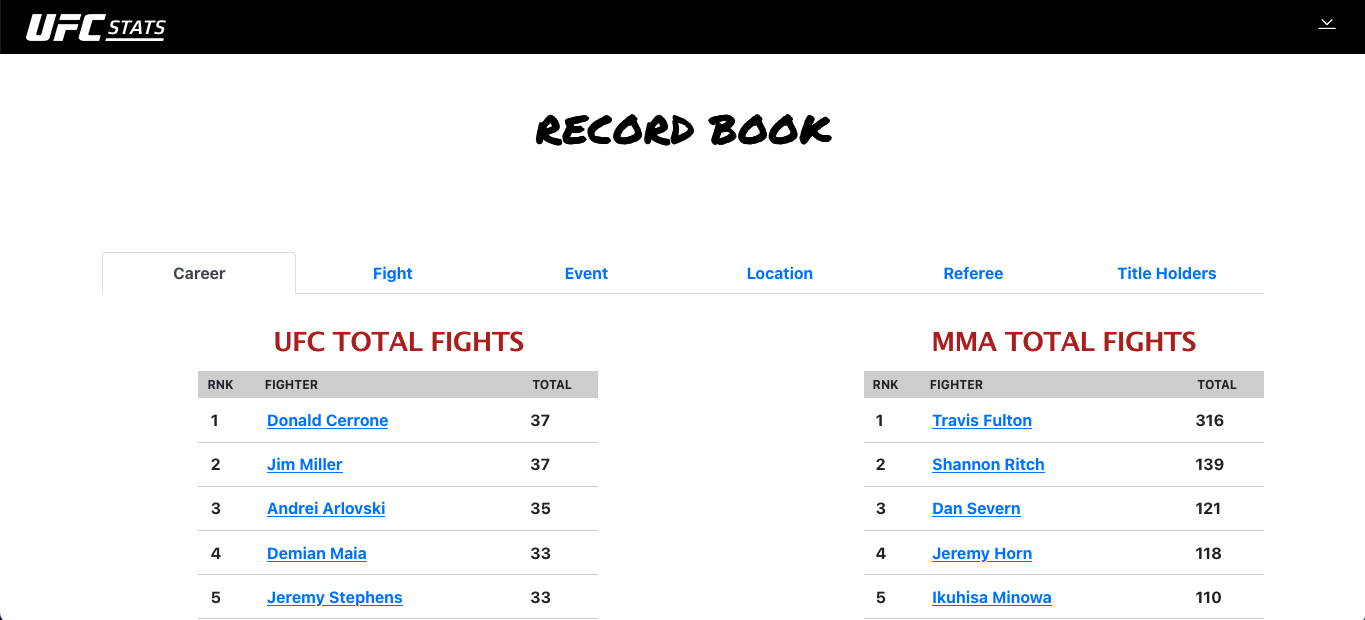
\includegraphics[width=1\textwidth]{imagens/Stats/Career Stats.png}
    \caption{Career Stats}
    \label{fig:mesh1}
\end{figure}

\begin{figure}[H]
    \centering
    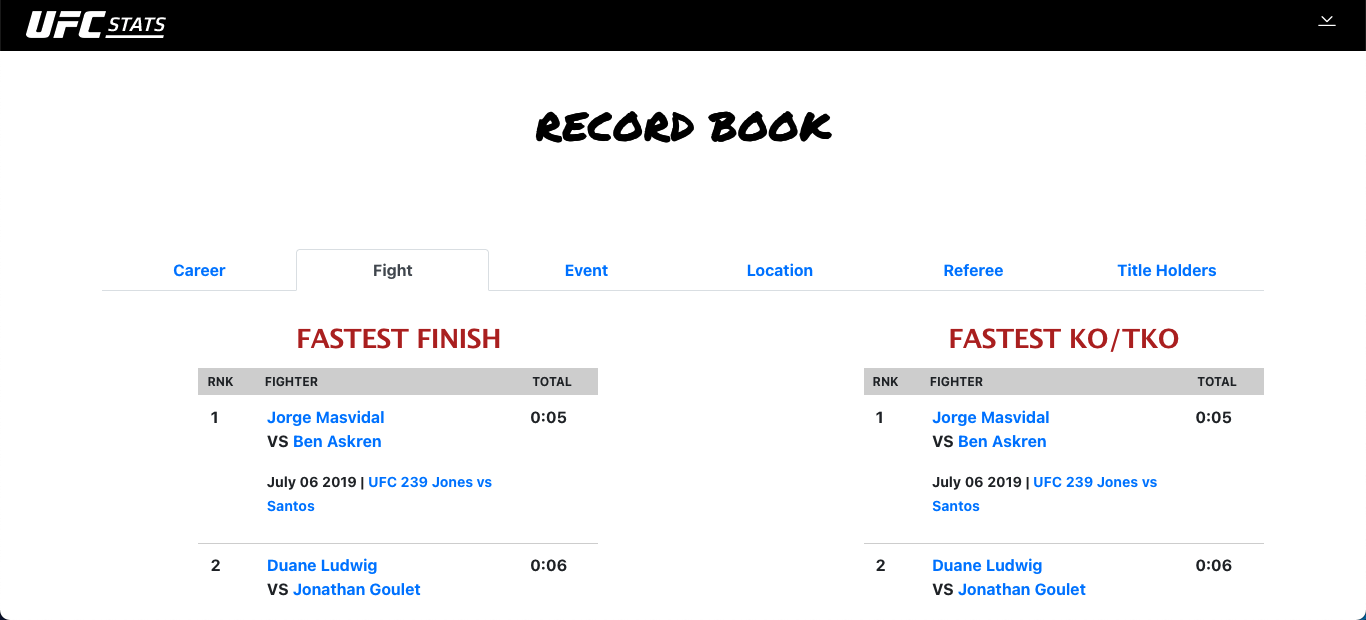
\includegraphics[width=1\textwidth]{imagens/Stats/Fight Stats.png}
    \caption{Fight Stats}
    \label{fig:mesh1}
\end{figure}


\begin{figure}[H]
    \centering
    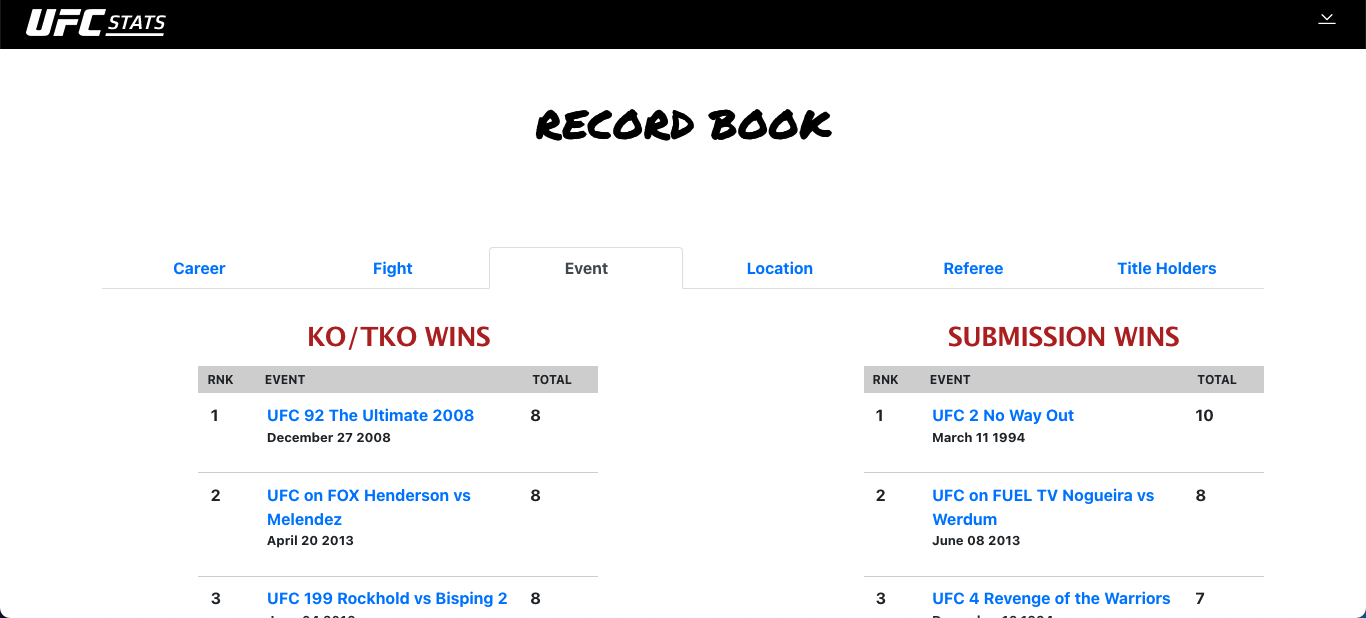
\includegraphics[width=1\textwidth]{imagens/Stats/Event Stats.png}
    \caption{Event Stats}
    \label{fig:mesh1}
\end{figure}



\begin{figure}[H]
    \centering
    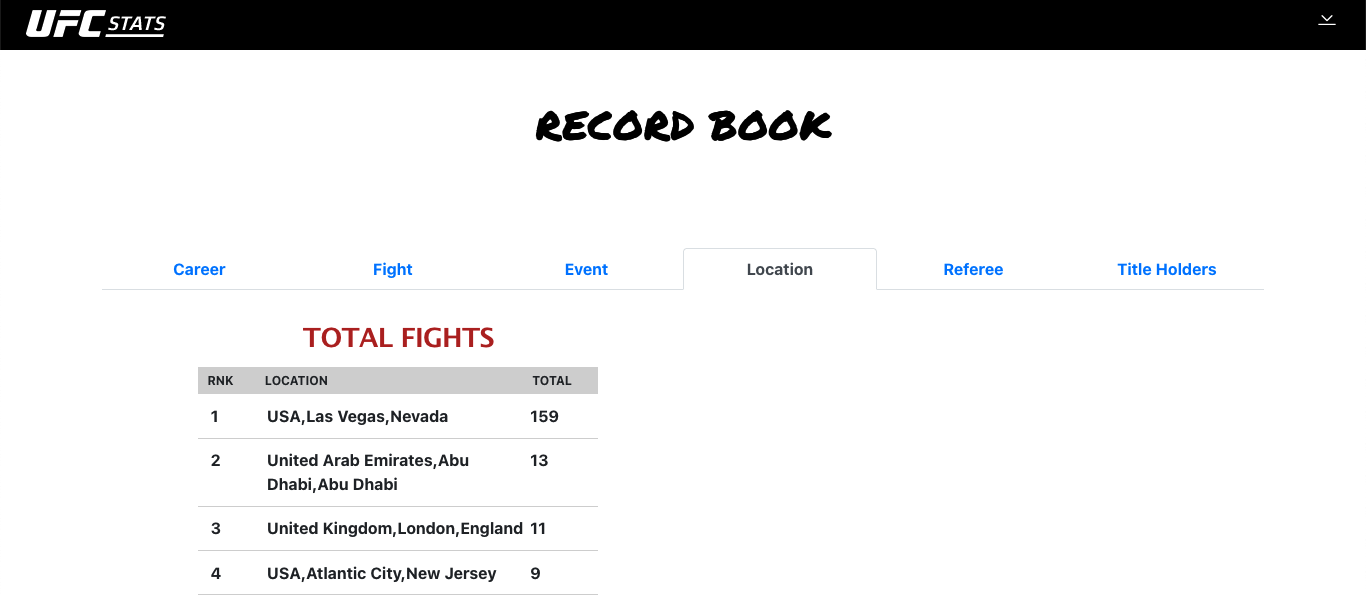
\includegraphics[width=1\textwidth]{imagens/Stats/Location Stats.png}
    \caption{Location Stats}
    \label{fig:mesh1}
\end{figure}


\begin{figure}[H]
    \centering
    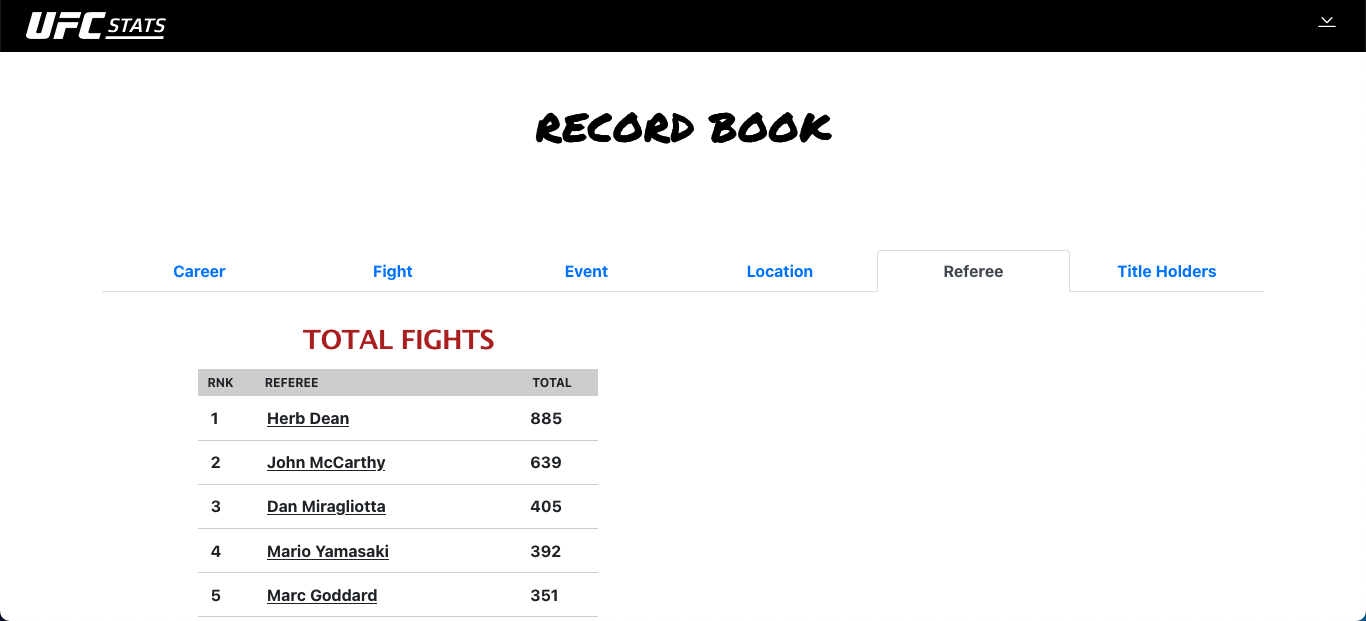
\includegraphics[width=1\textwidth]{imagens/Stats/Referee Stats.png}
    \caption{Referee Stats}
    \label{fig:mesh1}
\end{figure}

\begin{figure}[H]
    \centering
    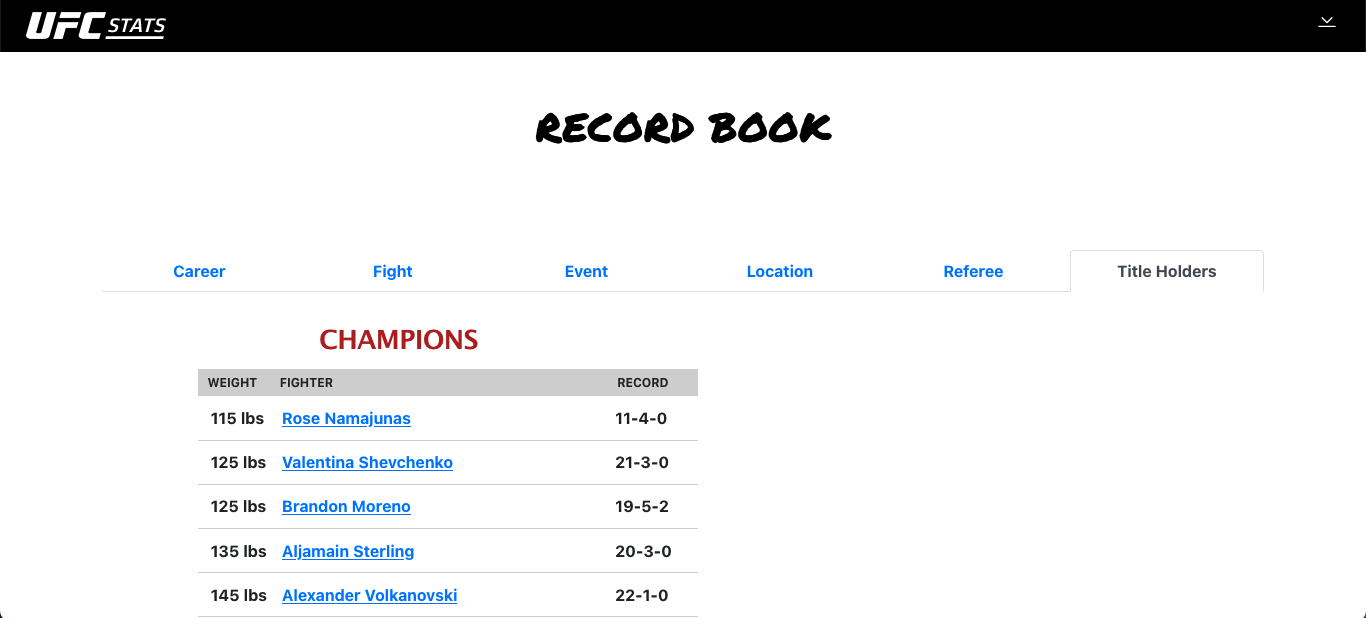
\includegraphics[width=1\textwidth]{imagens/Stats/Title Holders.png}
    \caption{Title Holders}
    \label{fig:mesh1}
\end{figure}


\begin{figure}[H]
    \centering
    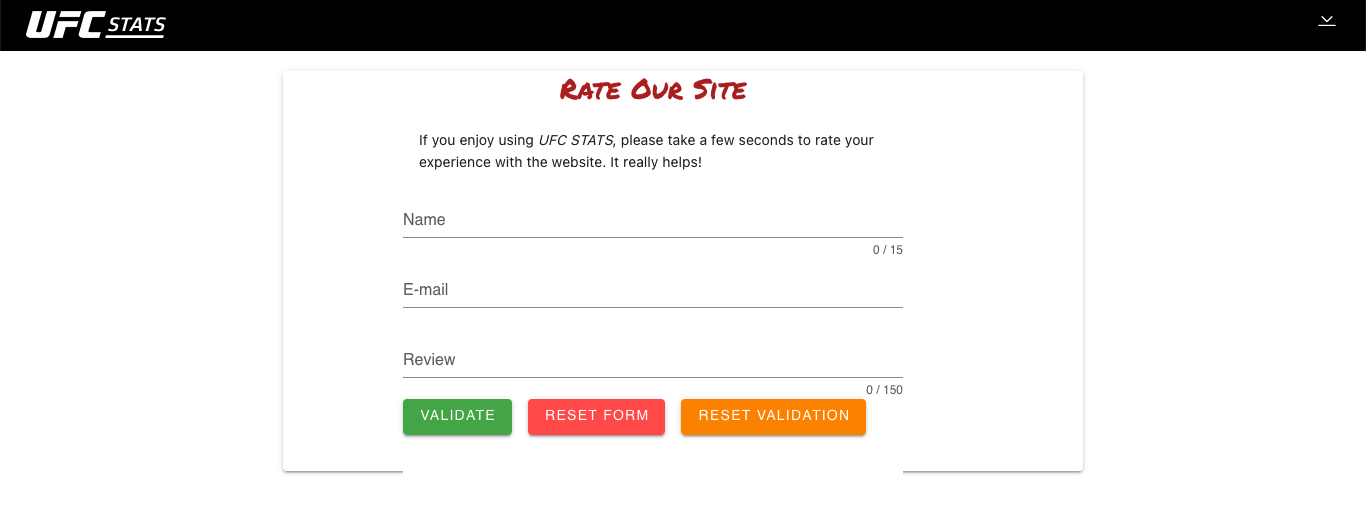
\includegraphics[width=1\textwidth]{imagens/Reviews/Rate.png}
    \caption{Rate Us}
    \label{fig:mesh1}
\end{figure}

\begin{figure}[H]
    \centering
    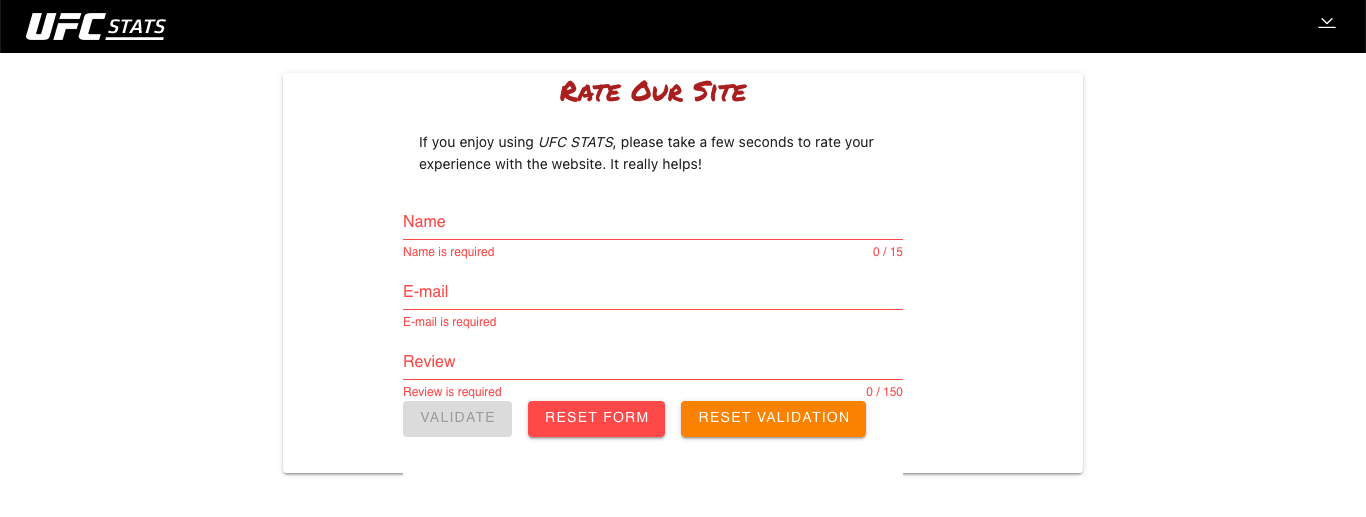
\includegraphics[width=1\textwidth]{imagens/Reviews/Rate Error.png}
    \caption{Rate Error}
    \label{fig:mesh1}
\end{figure}


\begin{figure}[H]
    \centering
    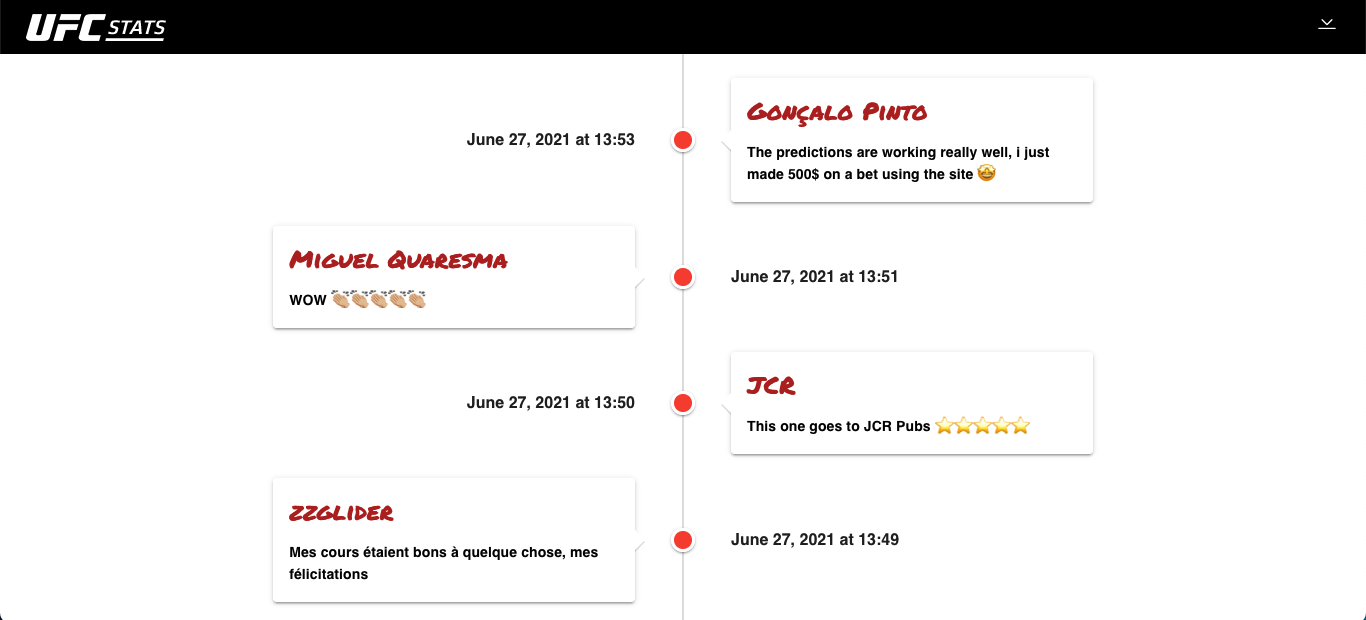
\includegraphics[width=1\textwidth]{imagens/Reviews/Reviews.png}
    \caption{Reviews}
    \label{fig:mesh1}
\end{figure}

\begin{figure}[H]
    \centering
    
\includegraphics[width=1\textwidth]{imagens/Structure/Repositorie Details.png}
    \caption{Ontology Details}
    \label{fig:mesh1}
\end{figure}

\begin{figure}[H]
    \centering
    
\includegraphics[width=1\textwidth]{imagens/Special Efects/PageNotFound.png}
    \caption{Page Not Found }
    \label{fig:mesh1}
\end{figure}



\newpage
\section{How to start}

De modo a facilitar a execução completa do projecto, criou-se um pequeno script
\textit{ufc-script.scpt} compilado criado com o editor de scripts da Apple.
Ele é escrito em AppleScript, uma linguagem de script de automação usada por computadores Mac, sendo que os mesmos podem ser gravados manualmente ou gerados por acções de gravação .

Para tirar partido desse script desenvolvido , existe a necessidade de resolver algumas dependências : 

\begin{itemize}
    \item iTerm - Terminal utilizado pelos criadores do sistema .
    \item Node.js
    \item Nodemon
    \item GraphDB
\end{itemize}

O comando de execução é o seguinte : \textbf{osascript ufc-script.scpt}

\begin{lstlisting}[language=python, caption= ufc-script.scpt]
tell application "iTerm"
	--Create initial window
	create window with default profile
	
	--Create fours tab in the initial window
	tell current window
			create tab with default profile
	        create tab with default profile
			create tab with default profile
	end tell

	--API SERVER
	tell current session of tab 1 of current window
		write text "cd /Users/etiennecosta/Desktop/Mestrado/PLC/PRC/UFC-PREDICTIONS/ufc-api"
		write text "nodemon npm run start"
	end tell
	

	--MongoDB SERVER
	tell current session of tab 2 of current window
		write text "cd /Users/etiennecosta/Desktop/Mestrado/PLC/PRC/UFC-PREDICTIONS/ufc-mongodb"
		write text "nodemon npm run serve"
	end tell

	--APP SERVER
	tell current session of tab 3 of current window
		write text "cd /Users/etiennecosta/Desktop/Mestrado/PLC/PRC/UFC-PREDICTIONS/ufc-app"
		write text "npm run serve"
	end tell

	--RUN GraphDB
	tell current session of tab 4 of current window
		write text "open  /Applications/'GraphDB Free.app' "
	end tell

end tell

\end{lstlisting} 





\section{Deployment}

De modo a tornar a aplicação acessível à comunidade interessada, decidiu-se recorrer ao \textit{Docker}. 
O Docker é um conjunto de produtos de plataforma como serviço que usam virtualização de nível de sistema operativos para entregar software em pacotes chamados containers. Os containers são isolados uns dos outros e agrupam os seus próprios softwares, bibliotecas e arquivos de configuração. 

De seguida são relembrados os serviços implementados, tendo para cada um deles um \textit{Dockerfile associado}.

\subsection{GraphDB}

A criação e execução deste \textit{Dockerfile} permite-nos ter uma imagem do \textit{GraphDB} com a nossa ontologia sobre o ufc.


\begin{lstlisting}[language=python, caption= GraphDB Dockerfile ]
FROM openjdk:8-jdk

ARG version=free-9.8.0
ARG dataFile=ufc-inf.ttl

ENV GRAPHDB_PARENT_DIR=/opt/graphdb
ENV GRAPHDB_HOME=${GRAPHDB_PARENT_DIR}/home

ENV GRAPHDB_INSTALL_DIR=${GRAPHDB_PARENT_DIR}/dist

ENV UFC=${GRAPHDB_HOME}/data/repositories/UFC

ADD ./graphdb-${version}-dist.zip /tmp

RUN mkdir -p ${GRAPHDB_PARENT_DIR} && \
    cd ${GRAPHDB_PARENT_DIR} && \
    unzip /tmp/graphdb-${version}-dist.zip && \
    rm /tmp/graphdb-${version}-dist.zip && \
    mv graphdb-${version} dist && \
    mkdir -p ${GRAPHDB_HOME} && \
    mkdir -p ${UFC}

COPY ./UFC-config.ttl ${UFC}/config.ttl
COPY ./${dataFile} /tmp

RUN sed -i 's|# graphdb.home.data =|graphdb.home.data = ../home/data|' ${GRAPHDB_INSTALL_DIR}/conf/graphdb.properties

RUN /opt/graphdb/dist/bin/loadrdf -f -c ${UFC}/config.ttl -m parallel /tmp/${dataFile}

ENV PATH=${GRAPHDB_INSTALL_DIR}/bin:$PATH

CMD ["/opt/graphdb/dist/bin/graphdb", "-Dgraphdb.home=/opt/graphdb/home", "-s"]

EXPOSE 7200
\end{lstlisting} 

\begin{lstlisting}[language=python, caption= Ficheiro de configuração config.ttl ]
#
# RDF4J configuration template for a GraphDB Free repository
#
@prefix rdfs: <http://www.w3.org/2000/01/rdf-schema#>.
@prefix rep: <http://www.openrdf.org/config/repository#>.
@prefix sr: <http://www.openrdf.org/config/repository/sail#>.
@prefix sail: <http://www.openrdf.org/config/sail#>.
@prefix owlim: <http://www.ontotext.com/trree/owlim#>.

[] a rep:Repository ;
    rep:repositoryID "UFC" ;
    rdfs:label "UFC" ;
    rep:repositoryImpl [
        rep:repositoryType "graphdb:FreeSailRepository" ;
        sr:sailImpl [
            sail:sailType "graphdb:FreeSail" ;
            
            owlim:base-URL "http://example.org/owlim#" ;
            owlim:defaultNS "" ;
            owlim:entity-index-size "10000000" ;
            owlim:entity-id-size  "32" ;
            owlim:imports "" ;
        	owlim:repository-type "file-repository" ;
            owlim:ruleset "rdfsplus-optimized" ;
            owlim:storage-folder "storage" ;
 
            owlim:enable-context-index "false" ;

            owlim:enablePredicateList "true" ;

            owlim:in-memory-literal-properties "true" ;
            owlim:enable-literal-index "true" ;

            owlim:check-for-inconsistencies "false" ;
            owlim:disable-sameAs  "true" ;
            owlim:query-timeout  "0" ;
            owlim:query-limit-results  "0" ;
            owlim:throw-QueryEvaluationException-on-timeout "false" ;
            owlim:read-only "false" ;
        ]
    ].
\end{lstlisting} 

É de salientar que na directoria deve estar presente o \textit{turtle} que se pretende inserir, bem como uma distribuição do graphdb . 




\subsection{UFC API}

Dockerfile associado à API que tem como objectivo fazer as queries ao nosso servidor que contém a imagem do \textit{GraphDB}.

\begin{lstlisting}[language=python, caption= UFC-API Dockerfile]
FROM node:latest
WORKDIR /ufc-api
COPY . /ufc-api
RUN npm install
CMD ["npm", "start"]
\end{lstlisting} 

\newpage
\subsection{UFC Mongo}

Dockerfile associado à API que tem como objectivo fazer garantir a persistência de dados que não estão diretamente ligados a nossa ontologia .

\begin{lstlisting}[language=python, caption= UFC-Mongo Dockerfile]
FROM node:latest
WORKDIR /ufc-mongo
COPY . /ufc-mongo
RUN npm install
CMD ["npm", "start"]
EXPOSE 8078
\end{lstlisting} 



\subsection{UFC APP}



Dockerfile associado à aplicação desenvolvida.

\begin{lstlisting}[language=python, caption= UFC-APP Dockerfile]
FROM node:latest
COPY . /app
WORKDIR /app
RUN npm install && npm run build

FROM nginx
RUN mkdir /app
COPY --from=0 /app/dist /app
COPY nginx.conf /etc/nginx/nginx.conf
CMD ["nginx", "-g", "daemon off;"]
\end{lstlisting} 

\newpage
\begin{lstlisting}[language=python, caption= NGINX.conf File]

user  nginx;
worker_processes  1;
error_log  /var/log/nginx/error.log warn;
pid        /var/run/nginx.pid;
events {
  worker_connections  1024;
}
http {
  include       /etc/nginx/mime.types;
  default_type  application/octet-stream;
  log_format  main  '$remote_addr - $remote_user [$time_local] "$request" '
                    '$status $body_bytes_sent "$http_referer" '
                    '"$http_user_agent" "$http_x_forwarded_for"';
  access_log  /var/log/nginx/access.log  main;
  sendfile        on;
  keepalive_timeout  65;
  server {
    listen       7777;
    server_name  localhost;
    location / {
      add_header 'Access-Control-Allow-Origin' '*';
      add_header 'Access-Control-Allow-Methods' 'GET, POST, PUT, DELETE, OPTIONS';
      add_header 'Access-Control-Allow-Headers' 'Accept,Authorization,Cache-Control,Content-Type,DNT,
      If-Modified-Since,Keep-Alive,
      Origin,User-Agent,X-Requested-With,Content-Length';
      if ($request_method = 'OPTIONS') {
        add_header 'Access-Control-Max-Age' 1728000;
        add_header 'Content-Type' 'text/plain; charset=utf-8';
        add_header 'Content-Length' 0;
        return 204;
      }
      root   /app;
      index  index.html;
      try_files $uri $uri/ /index.html;
    }
    error_page   500 502 503 504  /50x.html;
    location = /50x.html {
      root   /usr/share/nginx/html;
    }
  }
}

\end{lstlisting} 
\newpage
\subsection{Docker Compose}

Compose é uma ferramenta para definir e executar aplicativos Docker de vários containers. Com o Compose,usa-se um arquivo YAML para configurar os serviços das aplicações. 

Portanto aos interessados em correr a aplicação, basta terem instaladas as dependências \textit{Docker} e \textit{Docker-Compose} e executar :

\begin{lstlisting}[language=python, caption=docker-compose command]
 docker-compose -f docker-compose.yml up
\end{lstlisting}

\begin{lstlisting}[language=python, caption=docker-compose.yml]
version: '3'
services:
  mongo:
    image: mongo
    volumes:
      - db-data:/data/db
    ports:
      - "27017:27017"
  graphdb-ufc:
    image: etiennecosta/graphdb-ufc
    ports:
      - "7200:7200"
  sparql-api-ufc:
    image: etiennecosta/sparql-api-ufc:latest
    restart: on-failure
    links:
      - graphdb-ufc
    ports:
      - "8079:8079"
  mongodb-ufc:
    image: etiennecosta/mongodb-ufc
    restart: on-failure
    links:
      - mongo
    ports:
      - "8078:8078"
  interface-vue-ufc:
    image: etiennecosta/interface-vue-ufc
    links:
      - mongodb-ufc
    ports:
      - "8080:7777"
volumes:
  db-data:
\end{lstlisting} 


\newpage



\section{Conclusion} \label{sec:conclusao}

O processo de realização deste projecto foi dividido em diversas etapas, tendo cada uma a sua complexidade associada, mas apesar das dificuldades encontradas durante a realização conseguiu-se implementar na totatilidade todas as funcionalidades desejadas. Todo software está passível de melhorias, portanto, como trabalho futuro  seria desejável ter a capacidade de executar o script de criação e integração  semanalmente de modo a garantir que a informação esteja sempre actualizada, e também será desenvolvido o próprio algoritmo de previsão de modo a que os utilizadores registem uma versão sua de lutador e tentar prevar os resultados com os diversos lutadores da companhia .


\newpage
\begin{thebibliography}{8}

\bibitem{ref_urlMongo}
MongoDB Homepage, \url{http://www.MongoDB.com}. 
\bibitem{ref_urlNodeJS}
Nodejs Homepage, \url{https://nodejs.org/en/}.
\bibitem{ref_urlVueJS}
Vue.js Homepage, \url{https://vuejs.org/}.
\bibitem{ref_urlVuetify}
Vuetify Homepage, \url{https://vuetifyjs.com/en/}. 
\bibitem{ref_urlufc}
UFC, \url{https://www.ufc.com/}. 

\bibitem{ref_urldocker}
Docker, \url{https://www.docker.com/}. 

\bibitem{ref_urlsparql}
SPARQL Query Language for RDF, \url{https://www.w3.org/TR/rdf-sparql-query/}



\end{thebibliography}

\end{document}